\documentclass[12pt]{report}

% \usepackage[utf8]{inputenc}
% \usepackage[T1]{fontenc}

% \usepackage[default]{fontsetup}
\usepackage{termes-otf}

% \usepackage{amsmath}
% \usepackage{amsthm}
% \usepackage{amssymb}

\usepackage[a4paper, margin=25mm]{geometry}

\usepackage{setspace} \onehalfspace

\usepackage[estonian]{babel}

\usepackage[hidelinks]{hyperref}

\usepackage{booktabs}

\usepackage{graphicx}

\usepackage{yquant} \useyquantlanguage{groups} \newcommand*{\yquanton}{}

\usepackage[sorting=none, style=numeric, maxbibnames=99]{biblatex}
\addbibresource{srcs.bib}

\def\paren#1{\left(#1\right)}
\def\sparen#1{\left[#1\right]}
\def\cparen#1{\left\{#1\right\}}

\def\abs#1{\left|#1\right|}

\def\d#1{\mathinner{d#1}}

\def\bra#1{\left<#1\right|}
\def\ket#1{\left|#1\right>}

\def\CNOT{\mathop{\rm CNOT}\nolimits}
\def\SWAP{\mathop{\rm SWAP}\nolimits}

\def\QFT{\mathop{\rm QFT}\nolimits}

\begin{document}

\begin{titlepage}
    \begin{center}
        \large
        {\sc Tartu Ülikool} \\
        Loodus- ja täppisteaduste valdkond \\
        Füüsika instituut \\


        \vspace{25mm}
        \Large Mattias Märka

        \vspace{4mm}
        \Huge Molekulaarse hamiltoniaani põhioleku energia leidmine faasi hindamise algoritmi abil

        \vspace{20mm}
        \Large Bakalaureusetöö (6 EAP) \\
        Füüsika, keemia ja materjaliteaduse õppekava \\
	Füüsika eriala \\

        \vspace{20mm}
        \begin{flushright}
            \Large Juhendaja: Veiko Palge, PhD
        \end{flushright}

        \vfill
        \large Tartu 2024
    \end{center}
\end{titlepage}

\newpage

\noindent\textbf{\large Molekulaarse hamiltoniaani põhioleku energia leidmine faasi hindamise algoritmi abil}

\vspace*{1ex}

\noindent\textbf{Lühikokkuvõte:}
On teada, et klassikalised meetodit kvantsüsteemide täpseks simuleerimiseks on oma olemuselt ebaefektiivsed, mis on takistanud nende kasutamist paljude ülesannete lahendamiseks.
Töös tutvustatakse kvantarvutusliku meetodit molekulaarse hamiltoniaani põhinerega leidmiseks, mis põhineb faasi hindamise algoritmil ja mis on klassikalisest efektiivsem.
Meetodit rakendatakse vesiniku molekuli põhienergia leidmiseks.
Esmalt tutvustatakse elektronstruktuuri ülesande teoreetilist tausta.
Järgmisena antakse ülevaade molekulaarse süsteemi hamiltoniaani põhienergia leidmiseks vajalikest vahenditst: Jordan-Wigneri teisendusest, trotteriseerimisest, treppalgoritmist ja faasi hindamise algoritmist.
Arvutused viiakse läbi kasutades kvantarvuti klassikalist simulaatorit.
Lõpuks käsitletakse vajalike parameetrite valikut ja ülesande lahendamise võimalikkust kvantarvutil.

\vspace*{1ex}

\noindent\textbf{Võtmesõnad:}
kvantarvutus, kvantkeemia, kvantalgoritmid, faasi hindamise algoritm, elektronstruktuuri ülesanne

\vspace*{1ex}

\noindent\textbf{CERCS:}
P190 Matemaatiline ja üldine teoreetiline füüsika, klassikaline mehaanika, kvantmehaanika, relatiivsus, gravitatsioon, statistiline füüsika, termodünaamika;
P410 Teoreetiline ja kvantkeemia

\vspace*{2ex}

\noindent\textbf{\large Computation of the ground state energy of a molecular hamiltonian using the quantum phase estimation algorithm}

\vspace*{1ex}

\noindent\textbf{Abstract}:
It is known that classical methods for the simulation of quantum systems are inherently inefficient.
In this work an overview is given of a quantum computational method for finding the groun dstate energy of a molecular hamiltonian, which uses the quantum phase estimation algorithm and is more efficient than any classical method.
The quantum computational method is used to calculate the ground state energy of the hydrogen molecule.
First, a introduction is given to the electronic structure problem.
Then, an overview is given of the quantum compuational methods used to solve the problem: namely the Jordan-Wigner decomposition, trotterization, staircase algorithm and phase estimation algorithm.
A classical simulator is used for the quantum computational calculations.
Finally, the choice of simulation parameters and possibility of using a quantum computer for the calculations is discussed.

\noindent\textbf{Keywords:}
quantum computing, quantum chemistry, quantum algorithms, quantum phase estimation algorithm, electronic structure problem

\vspace*{1ex}

\noindent\textbf{CERCS:}
P190 Mathematical and general theoretical physics, classical mechanics, quantum
mechanics, relativity, gravitation, statistical physics, thermodynamics; P410 Theoretical chemistry, quantum chemistry

\tableofcontents

\chapter{Sissejuhatus}

Kvantarvutuste valdkonna üks peamine arengumotivatsioon on alati olnud soov simuleerida keerulisi kvantsüteeme.
Juba 1980ndatel, kui valdkond oli alles tekkimas, käisid Juri Manin ja Richard Feynman teineteiest eraldi välja idee, et kvantsüsteemide simuleerimiseks võiksid hästi sobida just kvantarvutid~\cite{manin, feynman}.

Simuleerimine on füüsikalise süsteemi käitumise kindlaks tegemine arvutuslikult.
Simulatsiooniülesande saab analüütiliselt lahendada vaid lihtsaimate kvantsüsteemide jaoks, mille tuntuimad näited on harmooniline ostsillaator ja vesiniku aatom.
Keerukamate süsteemide klassikaliseks simuleerimiseks kasutatakse numbrilisi meetodeid~\cite{szabo+ostlund, whitfield+etal2011}.

Kvantsüsteemi simuleerimisülesande klassikaline lahendamine on aga möödapääsmatult ebaefektiivne: Schrödingeri võrrandi klassikalise lahendamise ressursikulu sõltub süsteemi suurusest eksponentsiaalselt~\cite{whitfield+etal2011, mcardle+etal, cao+etal, kassal+etal}.
Klassikaliselt ei pruugi suuremaid ülesandeid olla kunagi võimalik lahendada, ammugi täpselt.

Samas on teada mitu tähtsat kvantalgoritmi, mille teoreetiline efektiivsus ületab klassikalise analoogi oma.
Komplekssusteoorias öeldakse, et lahenduvad on need ülesanded, mille ressursikulu sõltub süsteemi suurusest polünoomiselt; lahendamatud on need ülesanded, mille ressursikulu sõltub süsteemi suurusest eksponentsiaalselt.
Mitmed klassikaliselt lahendamatud ülesanded on kvantarvutuslikult lahendatavad.
Arvatakse, et nende kvantarvutitega saab tulevikus lahendada ülesandeid, mille klassikalist lahendamist peetakse jäädavalt liiga kulukaks.
Need algoritmid on võimalikud tänu kvantarvutuse ainulaadsetele vahenditele.

Kvantsimulatsioon on kvantsüsteemide simuleerimine kvantarvutuslikult.
Et kvantarvuti on ju ka ise kvantsüsteem, siis on sellega võimalik soodsalt simuleerida uuritava kvantsüsteemi dünaamikat.
Seda arvasid juba Manin ja Feynman~\cite{manin, feynman}.
Eelis klassikalise simuleerimise ees on eksponentsiaalne~\cite{whitfield+etal2011, mcardle+etal, cao+etal}.

Siiani on kvantarvututitega õnnestunud lahendada vaid mõni üksik selline probleem, mille lahendamine on klassikaliste arvutitega on teoreetiliselt võimatu.
Nimelt takistab kvantarvutite kasutamist nende ebatäiuslik riistvara: arvutuste käigus tekib müra~\cite{whitfield+etal2022}.

Siiski on kvantalgoritme mõttekas uurida tuleviku tarvis, sest kvantarvutite riistvara areneb pidevalt.
Pretsedendiks on klassikaliste arvutite kiire areng.
Lähemas tulevikus võib õnnestuda kasutada hübriidalgoritme, mis põhinevad kvantarvutite ja klassikaliste arvutite koostööl~\cite{omalley+etal}.

Käesoleva töö eesmärgiks on demonstreerida klassikalisest efektiivsemat kvantarvutuslikku meetodit molekulaarse hamiltoniaani simuleerimiseks.
See meetod põhineb faasi hindamise algoritmil.
Süsteemiks on vesiniku molekul \(\rm H_2\), ülesandeks on põhienergia leidmin kui näide elektronstruktuuri ülesandest.

Lahendamine algab klassikaliste eelarvutustega, mida tutvustab peatükk~\ref{chap:qchem}.
Eelarvutuste tulemuseks on hamiltoniaan teise kvantiseerimise kujul.
Peatükk~\ref{chap:qcomp} käsitleb ülesande kvantarvutusliku lahendamist.
Sammud lahendamiseks on järgmised~\cite{whitfield+etal2011}.

\begin{enumerate}
    \item Teise kvantiseerimise kujul molekulaarne hamiltoniaan tuleb esitada kvantbittide ruumis.
    Seda käsitleb jaotis~\ref{sec:jw}.
    \item Kvantbittide ruumis esitatud molekulaarse hamiltoniaani põhjal tuleb koostada ajalise arengu operaator ja realiseerida see kvantväravana.
    Seda käsitleb jaotis~\ref{sec:qcirc}.
    \item Ajalise arengu operaatori omaväärtused saab leida kasutades faasi hindamise algoritmi.
    Seda käsitleb alepeatükk~\ref{sec:pea}.
\end{enumerate}
Selguse huvides on sammud tekstis esitatud vastupidises järjekorras.
Metoodikat ja tulemusi käsitleb peatükk~\ref{chap:results}.
Peatükk~\ref{chap:discussion} räägib kvantarvuti kasutamisest töös esitatud arvutuste läbiviimiseks.

\chapter{Elektronstruktuuri ülesanne}\label{chap:qchem}

Käesoleva töö eesmärgiks on leida Schödingeri võrrandist
\begin{align}\label{eq:schro}
    H \Psi = E \Psi
\end{align}
molekulaarse süsteemi põhienergia.
Kahtlemata on selleks tarvis teada, milline on elektronkatet iseloomustav hamiltoniaan \(H\).
Hiljem näeme, et samuti on vajalik põhioleku lainefunktsiooni $\Psi_0$ lähendus, kuid see ei pea olema täpne.
Selle peatüki teemaks on arvutused hamiltoniaani ja põhioleku lainefunktsiooni lähenduse leidmiseks.
Need arvutused on ülesande lahendamiseks vajalikud, kuid mitte töö põhiosa, sestap nimetame neid eelarvutusteks.
Peatükis on vaatluse all järgmised teemad.
Esiteks, alapeatükis~\ref{sec:molhamgen} esitame molekulaarse süsteemi hamiltoniaani üld\-kuju.
Järgmiseks, alapeatükis~\ref{sec:bornopen} lihtsustame seda hamiltoniaani Born-Oppenheimeri lähenduse abil.
Siis, alapeatükis~\ref{sec:hpsd} leiame lainefunktsiooni üldise kuju.
Edasi, alapeatükis~\ref{sec:hartfock} kasutame Hartree-Focki lähendust, et leida põhioleku lainefunktsiooni lähendus.
Viimaks, alapeatükis~\ref{sec:secquant} esitame ülesande teise kvantiseerimise kujul.
See peatükk põhineb peamiselt Szabo ja Ostlundi käsitlusel~\cite{szabo+ostlund}, aga ka Whitfieldi jt omal~\cite{whitfield+etal2011}.

\section{Molekulaarse hamiltoniaani üldkuju}\label{sec:molhamgen}

Molekulaarse süsteemi, milles on \(N\) elektroni ja \(M\) tuuma, hamiltoniaani üldkuju aatom\-ühikutes on
\begin{align}\label{eq:molham}
    H_\text{mol} =
    \underbrace{- \sum_{i = 1}^N \frac{1}{2} \nabla_i^2}_\text{(a)}
    \underbrace{- \sum_{A = 1}^M \frac{1}{2 M_A} \nabla_A^2}_\text{(b)}
    \underbrace{- \sum_{i = 1}^N \sum_{A = 1}^M \frac{Z_A}{r_{iA}}}_\text{(c)}
    \underbrace{+ \sum_{i = 1}^N \sum_{j > i}^N \frac{1}{r_{ij}}}_\text{(d)}
    \underbrace{+ \sum_{A = 1}^M \sum_{B > A}^M \frac{Z_A Z_B}{r_{AB}}}_\text{(e)} \rlap{,}
\end{align}
kus \(M_A\) on tuuma \(A\) ja elektroni massi suhe, \(Z_A\) on tuuma \(A\) aatomnumber, \(r_{ij}\) on elektronide \(i\) ja \(j\) vahekaugus ning \(R_{AB}\) on tuumade \(A\) ja \(B\) vahekaugus.
Kutsume hamiltoniaani~\eqref{eq:molham} edaspidi molekulaarseks hamiltoniaaniks.
Selles esinevad järgmised liikmed: (a) on elektronide kineetilise energia liige, (b) on tuumade kineetilise energia liige, (c) on elektronide ja tuumade tõmbumise liige, (d) on elektronide omavahelise tõukumise liige ja (e) on tuumade omavahelise tõukumise liige.

Üldine hamiltoniaan~\eqref{eq:molham} kirjeldab nii elektronide kui ka tuumade dünaamikat, kuid kvantkeemia seisukohalt on enamasti oluline vaid elektronide dünaamika.
Eeldusel, et tuumade dünaamika pole oluline, on võimalik hamiltoniaani~\eqref{eq:molham} oluliselt lihtsustada, mida käsitlebki järgmine alapeatükk~\ref{sec:bornopen}.

\section{Born-Oppenheimeri lähendus}\label{sec:bornopen}

Et tuumade massid on palju suuremad kui elektronide massid, siis liiguvad tuumad palju aeglasemalt kui elektronid.
Kvantkeemias kasutatakse laialdaselt Born-Oppenheimeri lähendust, mille järgi on tuumad paigal.
Kasutame seda lähendust ka siin töös.

Born-Oppenheimeri lähendus lubab molekulaarset hamiltoniaani~\eqref{eq:molham} lihtsustada.
Esiteks võib arvestamata jätta kineetilise energia liikme (b), sest see on ligikaudu null.
Teiseks võib arvestamata jätta tuumade omavahelise tõmbumise liikme (e), sest see on konstantne.
Tulemuseks on vaid elektronide dünaamikat kirjeldav hamiltoniaan
\begin{align}\label{eq:elham}
    H_\text{elek} =
    \underbrace{- \sum_{i = 1}^N \frac{1}{2} \nabla_i^2}_\text{(a)}
    \underbrace{- \sum_{i = 1}^N \sum_{A = 1}^M \frac{Z_A}{r_{iA}}}_\text{(c)}
    \underbrace{+ \sum_{i = 1}^N \sum_{j > i}^N \frac{1}{r_{ij}}}_\text{(d)} \rlap{,}
\end{align}
mida kutsume elektrooniliseks hamiltoniaaniks.
Konstantse liikme~(e) arvestamata jätmise tõttu erinevad elektrooniline hamiltoniaan~\eqref{eq:elham} ja molekulaarne hamiltoniaan~\eqref{eq:molham} küll omaväärtuste poolest, kuid mitte omafunktsioonide poolest.
Täpsemalt öeldes kehtib seos
\begin{align}\label{eq:eigenelvsmol}
    E_\text{mol} = E_\text{elek} + E_\text{tuum} \rlap{,}
\end{align}
kus \(E_\text{mol}\) ja \(E_\text{elek}\) on vastavalt molekulaarse hamiltoniaani~\eqref{eq:molham} ja elektroonilise hamiltoniaani~\eqref{eq:elham} omaväärtused mingi ühise omafunktsiooni ning \(E_\text{tuum}\) on konstant, mis on kõikide omafunktsioonide jaoks sama.
Füüsikaliselt tähendab viimane võrdus seda, et Born-Oppenheimeri lähendsuses erineb elektronkatte energia molekuli energiast konstantse tuumade energia võrra.
Edaspidi jätame ära alaindeksi "elek", kuivõrd meid huvitabki vaid elektronkate.

\section{Hartree korrutis ja Slateri determinant}\label{sec:hpsd}

Hamiltoniaan~\eqref{eq:elham} ei võta arvesse spinni, seega peab spinni arvestama lainefunktsioon.
Lainefunktsioonile \(\Psi\) ongi kaks tingimust.
Ühest küljest peab see rahuldama Schrödingeri võrrandit~\eqref{eq:schro}.
Teisalt peab see rahuldama antisümmeetria printsiipi
\begin{align}\label{eq:antisim}
    \Psi(\vec{x}_1, \ldots, \vec{x}_i, \ldots, \vec{x}_j, \ldots, \vec{x}_N) =
    -\Psi(\vec{x}_1, \ldots, \vec{x}_j, \ldots, \vec{x}_i, \ldots, \vec{x}_N) \rlap{,}
\end{align}
kus \(\vec{x}_1\), \(\ldots\), \(\vec{x}_N\) on elektronide \(1\), \(\ldots\), \(N\) üldised koordinaadid.
Üldine kordinaat on
\begin{align}
    \vec{x} = (\vec{r}, \omega) \rlap{,}
\end{align}
kus \(\vec{r}\) on ruumiline kordinaat ja \(\omega\) spinn.
Antisümmeetria printsiip on Pauli keeluprintsiibi üldisem sõnastus.

Sobivate omadustega lainefunktsiooni saab molekulaarorbitaalide teooriast.
Selles teoorias nimetatakse spinnorbitaaliks funktsiooni
\begin{align}\label{eq:spinorb}
    \chi_i(\vec{x}) = \begin{cases}
        \alpha(\omega) \phi_i(\vec{r})\text{,} & \text{kui \(i\) ei jagu \(2\)-ga} \rlap{,}\\
        \beta(\omega) \phi_{i-1}(\vec{r})\text{,} & \text{kui \(i\) jagub \(2\)-ga} \rlap{.} \\
    \end{cases}
\end{align}
Spinnorbitaal on ühe elektroniga süsteemi lainefunktsiooniks.
Funktsioon \(\alpha(\omega)\) vastab spinn-alla seisundile ning \(\beta(\omega)\) spinn-üles seisundile.
Funktsioonid \(\cparen{\phi_j \middle| j = 1,2, \ldots, K}\) on ruumilised orbitaalid (mis ei arvesta spinni).
Iga ruumilise orbitaali kohta on kaks spinn\-orbitaali.
Spinnorbitaalide korrutist
\begin{align}
    \Psi^\text{HP}(\vec{x}_1, \vec{x}_2, \cdots, \vec{x}_N) =
    \chi_i(\vec{x}_1) \chi_j(\vec{x}_2) \cdots \chi_k(\vec{x}_N)
\end{align}
nimetatakse Hartree korrutiseks.
Kui antisümmeetria printsiipi poleks vaja arvestada, siis oleks Hartree korrutis \(N\)-i teineteisega mitteinterakteeruva elektroni süsteemi lainefunktsiooniks.
Sellisel lihtsustatud juhul oleksid elektronid sõltumatud: süsteemi hamiltoniaani saaks kirja panna kujul
\begin{align}
    H = \sum_i^N h(i) \rlap{,}
\end{align}
kus \(h(i)\) oleks üksiku elektroni hamiltoniaan.
Et kehtiks
\begin{align}
    E = \sum_j^N \epsilon_j \rlap{,}
    \qquad \text{kus} \qquad
    H \Psi^\text{HP} = E \Psi^\text{HP}
    \quad \text{ja} \quad
    h(i) \chi_j(\vec{x_i}) = \epsilon_j \chi_j(\vec{x_i}) \rlap{,}
\end{align}
siis sellise süsteemi koguenergia oleks üksikute elektronide energiate summa, mis näitab Hartree korrutise sobivust lainefunktsiooniks mitme elektroniga süsteemi lihtsustatud juhul.

Antisümmeetria printsiipi ja elektronide vastasmõju arvestab Slateri determinant
\begin{align}\label{eq:slater}
    \Psi(\vec{x_1}, \vec{x_2}, \ldots, \vec{x_n}) =
    \frac{1}{\sqrt{N!}} \begin{vmatrix}
        \chi_i(\vec{x_1}) & \chi_j(\vec{x_2}) & \cdots & \chi_k(\vec{x_2}) \\
        \chi_i(\vec{x_2}) & \chi_j(\vec{x_2}) & \cdots & \chi_k(\vec{x_2}) \\
        \vdots & \vdots & & \vdots \\
        \chi_i(\vec{x_N}) & \chi_j(\vec{x_N}) & \cdots & \chi_k(\vec{x_N}) \\
    \end{vmatrix} \rlap{.}
\end{align}
Slateri determinant on füüsikaliselt sobiv elektrooniline lainefunktsioon tulenevalt determinantide omadustest.

\section{Hartree-Focki lähendus}\label{sec:hartfock}

Kui hamiltoniaan~\eqref{eq:molham} on arvutamiseks liiga keeruline, siis kastutakse klassikalises kvantkeemias arvutusressursside kokku hoidmiseks Hartree-Focki lähendust.
Selles töös on Hartree-Focki lähendus vajalik vaid eelarvutuste läbiviimiseks: see lähendus lubab leida spinnorbitaalid \(\cparen{\chi_j | j=1, 2, \ldots, 2K}\), mis on vajalikud teise kvantiseerimise kuju leidmiseks, nagu selgub järgmises alapeatükis~\ref{sec:secquant}.

Hamiltoniaan~\ref{eq:molham} puhul on tegu mitme keha probleemiga.
Ülesande lihtsustamiseks eeldatakse Hartree-Focki lähenduses, et iga elektron liigub efektiivses väljas, mis saadakse teiste elektronide mõjude keskmistamisel.
Matemaatiliselt tähendab see järgmist.

Elektroonilise lainefunktsiooni üldkuju on~\eqref{eq:slater}.
Variatsiooniprintsiibist tulenevalt on põhioleku lainefunktsioon \(\Psi_0\) selline, mille energia
\begin{align}
    E_0 = \bra{\Psi_0} H \ket{\Psi_0}
\end{align}
on minimaalne.
Energia väärtus sõltub spinnorbitaalide valikust.
Minimeerimine viib Hartree-Focki võrrandini
\begin{align}
    f(i) \chi(\vec{x}_i) = \epsilon \chi(\vec{x}_i) \rlap{,}
\end{align}
kus
\begin{align}
  f(i) = -\frac{1}{2} \nabla_i^2 - \sum_{A = 1}^M \frac{Z_A}{r_{iA}} + v^\text{HF}(i)
\end{align}
on Focki operaator.
Liige \(v^\text{HF}\) on keskmine potentsiaal, mida kogeb üks elektron teiste elektronide tõttu.
Lahendamise tulemuseks on Hartree-Focki spinnorbitaalide komplekt \(\cparen{\chi_i \middle| i = 1, 2, \ldots}\), millele vastab energiate komplekt \(\cparen{\epsilon_i \middle| i = 1, 2, \ldots}\).

Need \(N\) spinnorbitaali, mis lainefunktsioonis esinevad, on täidetud orbitaalid; need, mis ei esine, on täitmata orbitaalid.
Põhiolekus on täidetud vaid madalaima energiaga orbitaalid.

Hartree-Focki võrrandil on lõpmata palju lahendeid: tulemuseks on lõpmata palju spinnorbitaale.
Praktikas valitakse arvutamiseks siiski lõpliku suurusega baasifunktsioonide komplekt $\cparen{\phi_i \middle| i = 1, 2, \ldots, K}$, mille tulemusena saadakse lõplik arv spinnorbitaale.
Baasifunktsioonide komplekti nimetatakse keemiliseks baasiks.
Väiksemad keemilised baasid on küll ebatäpsemad, kuid neid kasutades saab kokku hoida arvutusressursse.

\section{Teine kvantiseerimine}\label{sec:secquant}

Kui võimalik, kasutatakse kvantkeemias arvutamiseks teise kvantiseerimise kuju, milles lainefunktsiooni esitus on kompaktsem.
Selles töös on oluline, et teise kvantiseerimise kuju on vajalik lainefunktsiooni kujutamiseks kvantbittide ruumi, mis on teemaks alapeatükis~\ref{sec:jw}.

Teise kvantiseerimise formalismis esitatakse lainefunktsioon täitearvude esituses
\begin{align}
    \Psi(\vec{x}_1, \vec{x}_2, \ldots, \vec{x}_N) =
    \ket{\chi_1 \chi_2 \cdots \chi_{2K}} \rlap{,}
\end{align}
kus \(\chi \in \cparen{0, 1}\) viitab vastavalt täitmata või täidetud orbitaalile.
Selline lainefunktsiooni esitus on kompaktsem kui esitus Slateri determinandina, kuid antisümmeetria printsiibi kehtimisele tuleb pöörata eraldi tähelepanu.

Teise kvantiseerimise formalismis võetakse antisümmeetria printsiipi arvesse algebraliselt.
Selleks defineeritakse kaks sobivate omadustega operaatorit: tekkeoperaator \(a_i^\dagger\) ja kaooperaator \(a_i\).
Tekkeoperaator \(a_i^\dagger\) tekitab süsteemi juurde elektroni spinnorbitaalile \(\chi_i\):
\begin{align}
    a_i^\dagger \ket{\chi_k \cdots \chi_l} = \ket{\chi_i \chi_k \cdots \chi_l} \rlap{.}
\end{align}
Kaooperaator \(a_i\) eemaldab süsteemist elektroni spinnorbitaalilt \(\chi_i\):
\begin{align}
    a_i \ket{\chi_i \chi_k \cdots \chi_l} = \ket{\chi_k \cdots \chi_l}\rlap{.}
\end{align}
Kehtivad kommutatsioonireeglid
\begin{align}\label{eq:comrules}
    \sparen{a_i^\dagger, a_j^\dagger} = 0 \rlap{,}
    \qquad \sparen{a_i, a_j} = 0 \rlap{,}
    \qquad \sparen{a_i, a_j^\dagger} = \delta_{ij} \rlap{.}
\end{align}

Tekke- ja kaoperaatorite kaudu saab hamiltoniaani esitada teise kvantiseerimise kujul järgmiselt,
\begin{align}
    H = \sum_{pq}h_{pq}a_p^\dagger a_q
    + \frac{1}{2} \sum_{pqrs} a_p^\dagger a_q^\dagger a_r a_s \rlap{,}
\end{align}
kus
\begin{align}\label{eq:molint1}
    h_{pq} = \int\d{\vec{x}_i} \chi_p^*(\vec{x}_i)
    \paren{-\frac{1}{2} \nabla^2 - \sum_A \frac{Z_a}{r_{iA}}} \chi_q(\vec{x}_i)
\end{align}
ja
\begin{align}\label{eq:molint2}
    h_{pqrs} = \int \d{\vec{x}_1} \d{\vec{x}_2}
    \frac{\chi_p^*(\vec{x}_1) \chi_q^*(\vec{x}_2) \chi_r(\vec{x}_2) \chi_s(\vec{x}_1)}{r_{12}}
\end{align}
on molekulaarsed integraalid, mis seovad hamiltoniaani esimese ja teise kvantiseerimise kuju.
Need integraalid saab arvutada klassikaliselt.
Antud töös ongi ülesande lahendamise eelarvutuseks integraalide \eqref{eq:molint1} ja \eqref{eq:molint2} leidmine.

\chapter{Kvantarvutuslik lahendamine}\label{chap:qcomp}

\section{Põhimõisted}

Selles töös kasutame kvantarvutuse ahelamudelit, mille põhimõisted on kvantbitt ja kvantvärav.
Kvantahelamudel sarnaneb üldpildis klassikalisele ahelamudelile.
Järgneb kvantahelamudeli lühike ülevaade, mis lähtub Nielseni ja Chuangi~\cite{nielsen+chuang}; Kaye, Laflamme'i ja Mosca~\cite{kaye+laflamme+mosca} ning Whitfield jt  \cite{whitfield+etal2011, whitfield+etal2022} käsitlustest.

Kvantarvutuses on informatsiooni põhiühikuks kvantbitt, mis on Hilberti ruumi objekt.
Kõik kvantbiti olekud saab kirja panna kujul
\begin{align}
    \ket{\phi} = \alpha \ket{0} + \beta \ket{1} \rlap{,}
    \qquad \alpha, \beta \in \mathbb{C} \rlap{,}
    \qquad \abs{\alpha}^2 + \abs{\beta}^2 = 1 \rlap{,}
\end{align}
kus
\begin{align}\label{eq:compbasis}
    \ket{0} = \begin{pmatrix}
        1 \\
        0 \\
    \end{pmatrix} \rlap{,}
    \qquad
    \ket{1} = \begin{pmatrix}
        0 \\
        1 \\
    \end{pmatrix} \rlap{,}
\end{align}
on ortonormaalsed vektorid.
Siin töös kasutame kokkuleppeliselt Pauli \(Z\) operaatori omabaasi, mida nimetatakse arvutuslikuks baasiks.

Kvantbittide kogumit nimetatakse kvantregistriks ja selle olekuruum on üksikuid kvantbitte iseloomustavate Hilberti ruumide tensorkorrutis.
Kvantregistri jaoks on võimalikud kahte moodi olekud: korrutisolekud ja põimitud olekud.
Korrutisolekus saab lahutada üksikute kvantbittide olekuteks:
\begin{align}
    \ket{\Phi}
    = \ket{\phi_1} \otimes \ket{\phi_2} \otimes \cdots
    = \ket{\phi_1 \phi_2 \cdots} \rlap{,}
\end{align}
Põimitud olekut ei saa lahutada üksikute bittide olekuteks:
\begin{align}
    \ket{\Phi}
    \ne \ket{\phi_1 \phi_2 \cdots} \rlap{,}
\end{align}
Näide põimitud olekust on Belli olek
\begin{align}
    \frac{\ket{00} + \ket{11}}{\sqrt 2} \rlap{.}
\end{align}
Klassikalises teoorias põimitust ei esine.

Kvantväravad sooritavad kvantbittidel unitaarsed operatsioone.
Need võivad mõjutada ühte või rohkemat kvantbitti.
Mitut kvantbitti mõjutavad väravad võivad olla põimivad.
Siin töös kasutatud ühebitised väravad on toodud tabelis~\ref{tab:gates}
Võimalikke kvantväravaid on lõpmata palju, kuid riistvaras on vaja realiseerida vaid mõned väravad, mis moodustavad universaalse komplekti.
Kõik teised väravad saab esitada universaalse komplekti kaudu.
Universaalseid komplekte on lõpmata palju, kusjuures komplektis peab alati olema põimiv värav.
Antud töös kasutatakse põimimiseks juhitud eituse väravat.
Juhitud väravad on sellised, mis rakenduvad sihtbitile vaid siis, kui juhtbitt on olekus \(\ket1\), juhtibitti muutmata.
Näide juhitud eituse rakendamisest on järgmine,
\begin{align}
    \CNOT \paren{\alpha \ket{0} \otimes \ket{1} + \beta \ket{1} \otimes \ket{1}}
    = \alpha \ket{0} \otimes \ket{1} + \beta \ket{1} \otimes \ket{0} \rlap{,}
\end{align}
kus tensorkorrutise vasakul on juhtbitt ja paremal sihtbitt.
Töös kasutatud juhitud väravaid pole enamasti tabelis~\ref{tab:gates} eraldi toodud.
Mõõtmine pole unitaarne operatsioon ja sellega ei seostu väravat.
Siiski tähistatakse ahelates seda väravatega sarnaselt.

\begin{table}[]
    \centering
    \begin{tabular}{||c|c|c||}
        \toprule
        Operaator  & Maatriks & Tähis kvantahelas \\
        \midrule
        Pööre \(z\)-telje ümber \(R_z(\theta)\) & \(
        \begin{pmatrix}
            e^{-i\frac{\theta}{2}} & 0 \\
            0 & e^{i\frac{\theta}{2}} \\
        \end{pmatrix}
        \) & \lower6pt\hbox{
        \ifdefined\yquanton
        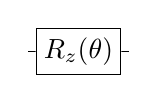
\begin{tikzpicture}
            \begin{yquant}
                qubit {} q[1];
                box {\(R_z(\theta)\)} q[0];
            \end{yquant}
        \end{tikzpicture}
        \fi} \\[1em]
        Faasinihe \(P(\lambda)\) & \(
        \begin{pmatrix}
            1 & 0 \\
            0 & e^{i\lambda} \\
        \end{pmatrix}
        \) & \lower6pt\hbox{
        \ifdefined\yquanton
        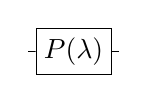
\begin{tikzpicture}
            \begin{yquant}
                qubit {} q[1];
                box {\(P(\lambda)\)} q[0];
            \end{yquant}
        \end{tikzpicture}
        \fi} \\[1em]
        Globaalse faasi nihe \(GP(\lambda)\) & \(
        \begin{pmatrix}
            e^{i\lambda} & 0 \\
            0 & e^{i\lambda} \\
        \end{pmatrix}
        \) & \lower6pt\hbox{
        \ifdefined\yquanton
        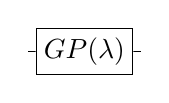
\begin{tikzpicture}
            \begin{yquant}
                qubit {} q[1];
                box {\(GP(\lambda)\)} q[0];
            \end{yquant}
        \end{tikzpicture}
        \fi} \\[1em]
        Juhitud eitus \(\CNOT\) & \(
        \begin{pmatrix}
            1 & 0 & 0 & 0 \\
            0 & 0 & 0 & 1 \\
            0 & 0 & 1 & 0 \\
            0 & 1 & 0 & 0 \\
        \end{pmatrix}
        \) & \lower6pt\hbox{
        \ifdefined\yquanton
        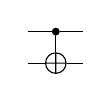
\begin{tikzpicture}
            \begin{yquant}
                qubit {} ctrl;
                qubit {} trgt;
                cnot trgt | ctrl;
            \end{yquant}
        \end{tikzpicture}
        \fi} \\
        Pauli \(X\) & \(
        \begin{pmatrix}
            0 & 1 \\
            1 & 0 \\
        \end{pmatrix}
        \) & \lower6pt\hbox{
        \ifdefined\yquanton
        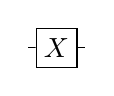
\begin{tikzpicture}
            \begin{yquant}
                qubit {} q[1];
                box {\(X\)} q[0];
            \end{yquant}
        \end{tikzpicture}
        \fi} \\[1em]
        Pauli \(Y\) & \(
        \begin{pmatrix}
            0 & -i \\
            i & 0 \\
        \end{pmatrix}
        \) & \lower6pt\hbox{
        \ifdefined\yquanton
        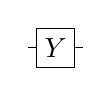
\begin{tikzpicture}
            \begin{yquant}
                qubit {} q[1];
                box {\(Y\)} q[0];
            \end{yquant}
        \end{tikzpicture}
        \fi} \\[1em]
        Pauli \(Z\) & \(
        \begin{pmatrix}
            1 & 0 \\
            0 & -1 \\
        \end{pmatrix}
        \) & \lower6pt\hbox{
        \ifdefined\yquanton
        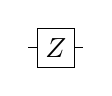
\begin{tikzpicture}
            \begin{yquant}
                qubit {} q[1];
                box {\(Z\)} q[0];
            \end{yquant}
        \end{tikzpicture}
        \fi} \\[1em]
        Hadamardi operaator \(H\) & \(
        \frac{1}{\sqrt{2}} \begin{pmatrix}
            1 & 1 \\
            1 & -1 \\
        \end{pmatrix}
        \) & \lower6pt\hbox{
        \ifdefined\yquanton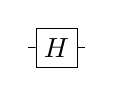
\begin{tikzpicture}
            \begin{yquant}
                qubit {} q[1];
                box {\(H\)} q[0];
            \end{yquant}
        \end{tikzpicture}
        \fi} \\[1em]
        Faasioperaator \(S\) & \(
        \begin{pmatrix}
            1 & 0 \\
            0 & i \\
        \end{pmatrix}
        \) & \lower6pt\hbox{
        \ifdefined\yquanton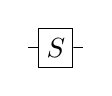
\begin{tikzpicture}
            \begin{yquant}
                qubit {} q[1];
                box {\(S\)} q[0];
            \end{yquant}
        \end{tikzpicture}
        \fi} \\[1em]
        Pöördfaasioperaator \(S^{\dagger}\) & \(
        \begin{pmatrix}
            1 & 0 \\
            0 & -i \\
        \end{pmatrix}
        \) & \lower6pt\hbox{
        \ifdefined\yquanton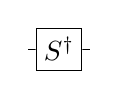
\begin{tikzpicture}
            \begin{yquant}
                qubit {} q[1];
                box {\(S^{\dagger}\)} q[0];
            \end{yquant}
        \end{tikzpicture}
        \fi} \\[1em]
        Bittide vahetus \(\SWAP\) & \(
        \begin{pmatrix}
            1 & 0 & 0 & 0 \\
            0 & 0 & 1 & 0 \\
            0 & 1 & 0 & 0 \\
            0 & 0 & 0 & 1 \\
        \end{pmatrix}
        \) & \lower6pt\hbox{
        \ifdefined\yquanton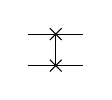
\begin{tikzpicture}
            \begin{yquant}
                qubit {} q[2];
                swap (q[0, 1]);
            \end{yquant}
        \end{tikzpicture}
        \fi} \\
        \midrule
        Mõõtmine & --- & \lower6pt\hbox{
        \ifdefined\yquanton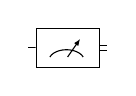
\begin{tikzpicture}
            \begin{yquant}
                qubit {} q[1];
                measure q[0];
            \end{yquant}
        \end{tikzpicture}
        \fi} \\
        \bottomrule
    \end{tabular}
    \caption{Töös kasutatud operaatorid, nende definitsioonid maatriksina ja tähistused ahelas.}
    \label{tab:gates}
\end{table}

Kvantäravate järjestuse ja bittidele rakendamise korra määrab kvantahel.
Joonisl~\ref{fig:circuits} on näide kvantahelast, mille lugemiseks tuleb arvestada järgmist.
Igat üksikut kvantbitti või -registrit tervikuna tähistab horisontaalne traat.
Traadist vasakul on sisend- ja paremal väljundolekud, kui need on olulised.
Operaatoreid tähitavad kastid.
Operaator rakendub igale kavantbitile, mille traat kasti läbib.
Katsutid (punktiga lõppevad vertikaalsed jooned) ühendavad operaatoreid juhtbittide või juhtregistritega, kui neid on.

\begin{figure}
    \centering
    \ifdefined\yquanton
    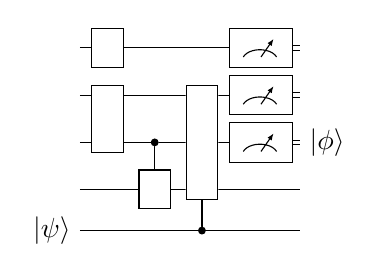
\begin{tikzpicture}
        \begin{yquant}
            qubit {} q[4];
            qubit {\(\ket{\psi}\)} q[+1];
            box {} q[0];
            box {} (q[1, 2]);
            box {} q[3] | q[2];
            box {} (q[1, 2, 3]) | q[4];
            measure q[0, 1, 2];
            output {\(\ket{\phi}\)} q[2];
        \end{yquant}
    \end{tikzpicture}
    \fi
    \caption{Näide kvantahelast.}
    \label{fig:circuits}
\end{figure}

\section{Faasi hindamise algoritm}\label{sec:pea}

Siin alapeatükis näitame, kuidas faasi hindamise algoritmi abil saab hinnata kvantbittide ruumis esitatud hamiltoniaani \(H\) omaväärtusi.
Esmalt, jaotises~\ref{sec:qftdef} tutvustama kvantarvutusliku Fourier' teisendust ja pöördteisendust, mis on faasi hindamise algoritmi tähtsad osad.
Järgmisena, jaotises~\ref{sec:unit} näitame, kuidas faasi hindamise algoritmiga on võimalik leida unitaarse operaatori omaväärtusi.
Viimaks, jaotises~\ref{sec:ham} kasutame faasi hindamise algoritmi hamiltoniaani omaväärtuste leidmiseks.
See alapeatükk toetub Nielseni ja Chuangi~\cite{nielsen+chuang}; Kaye, Laflamme'i ja Mosca~\cite{kaye+laflamme+mosca} ning Whitfield jt~\cite{whitfield+etal2011} käsitlusele.

\subsection{Kvantarvutuslik Fourier' teisendus ja pöördteisendus}\label{sec:qftdef}

Kvantarvutusliku Fourier' teisenduse algoritm ja pöördteisenduse algoritm on faasi hindamise algoritmi tähtsad osad.
Tutvustame neid.

Kvantarvutusliku Fourier' teisenduse definitsioon on
\begin{align}\label{eq:qftdef}
    \QFT\colon
    \ket{j} \mapsto \frac{1}{\sqrt{2^n}} \sum_{k=0}^{2^n-1} e^{2\pi ijk/2^n} \ket{k} \rlap{,}
\end{align}
kus \(\ket{j}\) ja \(\ket{k}\) \(n\)-kvantbitised baasivektorid.
Et tegemist on lineaarse operatsiooniga, siis piisab, kui käsitleda selle mõju baasivektoritele.

\begin{figure}
    \centering
    \ifdefined\yquanton
    \begin{tikzpicture}[scale=0.8]
        \begin{yquant}
            qubit {\(\ket{j_1}\)} q[1];
            qubit {\(\ket{j_2}\)} q[+1];
            qubit {\(\vdots\)} q[+1]; discard q[2];
            qubit {\(\ket{j_{n-1}}\)} q[+1];
            qubit {\(\ket{j_n}\)} q[+1];
            h q[0];
            box {\(P(2\pi/2^2)\)} q[0] | q[1];
            text {\(\ \ldots\ \)} q[0, 1, 3, 4];
            h q[1];
            text {\(\ \ldots\ \)} q[0, 1, 3, 4];
            box {\(P(2\pi/2^{n-2})\)} q[1] | q[3];
            box {\(P(2\pi/2^{n-1})\)} q[1] | q[4];
            text {\(\ \ldots\ \)} q[0, 1, 3, 4];
            h q[3];
            box {\(P(2\pi/2^2\)} q[3] | q[4];
            h q[4];
            swap (q[0, 4]);
            swap (q[1, 3]);
            output {\(\frac{\ket0+e^{2\pi0.j_n}\ket1}{\sqrt{2}}\)} q[0];
            output {\(\frac{\ket0+e^{2\pi0.j_{n-1}j_n}\ket1}{\sqrt{2}}\)} q[1];
            output {\(\vdots\)} q[2];
            output {\(\frac{\ket0+e^{2\pi0.j_2\cdots j_n}\ket1}{\sqrt{2}}\)} q[3];
            output {\(\frac{\ket0+e^{2\pi0.j_1\cdots j_n}\ket1}{\sqrt{2}}\)} q[4];
        \end{yquant}
    \end{tikzpicture}
    \fi
    \caption{Kvantarvutusliku Fourier' teisenduse ahel.}
    \label{fig:qft}
\end{figure}

Näitame, et kvantarvutusliku Fourier' teisenduse realiseerib ahel joonisel~\ref{fig:qft}.
Selleks on ilmekas kasutada tähistust
\begin{multline}
    j_1j_2\cdots j_n.j_{n+1}j_{n+2}\cdots j_m \\
    = j_1 2^{n-1} j_2 2^{n-2} + \cdots + j_n 2^0 + j_{n+1} 2^{-1} j_{n+2} 2^{-2} + \cdots j_m 2^{-m} \rlap{,}
    \qquad j_i \in \{0, 1\} \rlap{.}
\end{multline}
Teisisõnu, selles ja järgmisees jaotises on komaga arvud kahendmurrud, mitte kümnendmurrud.
Edasises on veel vaja teada, et Hadamardi operaatori mõju baasvektoritele on
\begin{align}
    H\ket{0} = \frac{\ket{0} + \ket{1}}{\sqrt{2}}
    \qquad\text{ja}\qquad
    H\ket{1} = \frac{\ket{0} - \ket{1}}{\sqrt{2}} \rlap{.}
\end{align}
Viimased kaks tingimust saab kokku võtta üheks
\begin{align}\label{eq:hprop}
    H\ket{j_i} = \frac{\ket{0} + e^{2\pi i0.j_i}\ket{1}}{\sqrt{2}}\rlap{.}
\end{align}
Samuti on vaja teada, et faasioperaatori mõju baasivektoritele on
\begin{align}
    P(\lambda)\ket{0} = \ket{0}
    \qquad\text{ja}\qquad
    P(\lambda)\ket{1} = e^{i\lambda}\ket{1} .
\end{align}
Viimasest kahest tingimusest järeldub kasulik omadus
\begin{align}\label{eq:phaseprop}
    P(2\pi i0.0j_2)\paren{\frac{\ket{0} + e^{2\pi i 0.j_1} \ket{1}}{\sqrt{2}}}
    = \frac{\ket{0}+e^{2\pi i0.j_1j_2}\ket{1}}{\sqrt{2}} .
\end{align}
Järgime nüüd joonise~\ref{fig:qft} ahelat samm-sammult.
Ahela alguses on kvantbitid olekus
\begin{align}
    \ket{j_1} \otimes \ket{j_2} \otimes \cdots \otimes \ket{j_n} \rlap{.}
\end{align}
Esimeses etapis rakendatakse esimesele kvantbitile Hadamardi operaatorit \(H\) ja seejärel faasioperaatoreid \(P(2\pi/2^2)\), \(P(\pi/2^3)\), \(\ldots\), \(P(\pi/2^4)\) juhinduvalt vastavalt teisest, kolmandast, \(\ldots\), \(n\)-ndast kvantbitist.
Hadamardi operaatori \(H\) rakendamise järel on olek
\begin{align}
    \frac{\ket{0} + e^{2\pi i0.j_1}\ket{1}}{\sqrt{2}} \otimes \ket{j_2} \otimes \cdots \otimes \ket{j_n}
\end{align}
tulenevalt valemist~\eqref{eq:hprop}.
Faasioperaatori \(P(2\pi/2^2) = P(2\pi0.01)\) rakendamise järel juhinduvalt teisest kvantbitist on olek
\begin{align}
    \begin{cases}
        \frac{\ket{0} + e^{2\pi i0.j_1}\ket{1}}{\sqrt{2}} \otimes \ket{j_2} \otimes \cdots \otimes \ket{j_n}\text{,} & \text{kui \(j_2 = 0\)} \rlap{,} \\
        \frac{\ket{0} + e^{2\pi i0.j_11}\ket{1}}{\sqrt{2}} \otimes \ket{j_2} \otimes \cdots \otimes \ket{j_n}\text{,} & \text{kui \(j_2 = 1\)} \rlap{,} \\
    \end{cases}
\end{align}
tulenevalt valmist~\eqref{eq:phaseprop}.
Viimase oleku kompaktsem kuju on
\begin{align}
    \frac{\ket{0} + e^{2\pi i0.j_1j_2}\ket{1}}{\sqrt{2}} \otimes \ket{j_2} \otimes \cdots \otimes \ket{j_n} \rlap{.}
\end{align}
Faasioperaatorite \(P(2\pi/2^3)\), \(P(2\pi/2^4)\), \(\ldots\), \(P(2\pi/2^n)\) rakendamise järel juhinduvalt vastavalt kolmandast, neljandast, \(\ldots\), \(n\)-ndast kvantbitist on olek
\begin{align}
   \frac{\ket{0} + e^{2\pi i0.j_1j_2\cdots j_n}\ket{1}}{\sqrt{2}} \otimes \ket{j_2} \otimes \cdots \otimes \ket{j_n} \rlap{,}
\end{align}
millega on esimene etapp lõppenud.
Järgmises etapis rakendatakse teisele kvantbitile Hadamardi operaatorit \(H\) ja seejärel faasioperaatoreid \(P(2\pi/2^2)\), \(P(2\pi/2^3)\), \(\ldots\), \(P(2\pi/2^{n-1})\) juhinduvalt kolmandast, neljandast, \(\ldots\) ja \(n\)-ndast kvantbitist.
Etapp on analoogne eelmise etapiga ja selle lõpuks on olek
\begin{align}
    \frac{\ket{0} + e^{2\pi i0.j_1j_2\cdots j_n}\ket{1}}{\sqrt{2}}
    \otimes \frac{\ket{0} + e^{2\pi i0.j_2j_3\cdots j_n}\ket{1}}{\sqrt{2}}
    \otimes \ket{j_3} \otimes \cdots \otimes \ket{j_n} \rlap{.}
\end{align}
Esimese ja teise kvantbiti jaoks läbitud etappidega sarnased etapid tuleb läbida ka ülejäänud kvantbittide jaoks, mille tulemuseks on olek
\begin{align}
    \frac{\ket{0} + e^{2\pi i0.j_1j_2\cdots j_n}\ket{1}}{\sqrt{2}}
    \otimes \frac{\ket{0} + e^{2\pi i0.j_2j_3\cdots j_n}\ket{1}}{\sqrt{2}}
    \otimes \cdots
    \otimes \frac{\ket{0} + e^{2\pi i0.j_n}\ket{1}}{\sqrt{2}} \rlap{.}
\end{align}
Ahela kõige viimases etapis vahetatakse kvantbittide järjekord.
Ahela lõpuks on olek
\begin{align}\label{f:qftfinal}
    \frac{\ket{0} + e^{2\pi i0.j_n}\ket{1}}{\sqrt{2}}
    \otimes \frac{\ket{0} + e^{2\pi i0.j_{n-1}j_n}}{\sqrt{2}}
    \otimes \cdots
    \otimes \frac{\ket{0} + e^{2\pi i0.j_1j_2\cdots j_n}\ket{1}}{\sqrt{2}} \rlap{.}
\end{align}
Avades sulud ja koondades saab viimase oleku kirja panna kujul
\begin{equation}\label{f:qftfinaltrans}
    \frac{1}{\sqrt{2^n}}\sum_{k=0}^{2^n-1}e^{2\pi ijk/2^n}\ket k \rlap{,}
\end{equation}
milline peabki olema kvantarvutusliku Fourier' teisenduse tulemus.

Järgnevas jaotises läheb vaja ka kvantarvutusliku Fourier' pöördteisendust, mille kohaselt
\begin{align}\label{eq:iqftdef}
    \QFT^{-1}\colon
    \frac{1}{\sqrt{2^n}} \sum_{k=0}^{2^n-1} e^{2\pi ijk/2^n} \ket{k} \mapsto \ket{j} \rlap{.}
\end{align}
Pöördteisenduse ahela saamiseks tuleb Fourier' teisenduse ahel pöörata: ahel tuleb koostada vastupidises järjekorras, asendades operaatorid pöördoperaatoritega, mille jaoks kehtivad seosed
\begin{align}
    H^{-1} &= H \rlap{,} \\
    P^{-1}(\lambda) &= P(-\lambda) \rlap{,} \\
    \SWAP^{-1} &= \SWAP \rlap{.}
\end{align}

\subsection{Unitaarse operaatori omaväärtuste leidmine}\label{sec:unit}

Unitaarse operaatori \(U\) jaoks kehtib omaväärtusvõrrand
\begin{align}\label{eq:uniteigen}
    U\ket{u} = e^{2\pi i\phi}\ket{u} \rlap{,}
    \qquad \phi \in [0,1) \rlap{,}
\end{align}
kus \(\ket{u}\) on meid huvitav olek ja \(e^{2\pi i\phi}\) omaväärtus, mida kutsutakse ka faasiks.
Faasi hindamise algoritm võimaldab leida parameetri \(\phi\), millega on faas määratud.

\begin{figure}[h]
    \centering
    \ifdefined\yquanton
    \begin{tikzpicture}
        \begin{yquant}
            qubit {$\ket0$} pea[1];
            qubit {$\ket0$} pea[+1];
            qubit {$\vdots$} pea[+1]; discard pea[2];
            qubit {$\ket0$} pea[+1];
            qubit {$\ket0$} pea[+1];
            qubit {$\ket u$} state;
            box {$\mathop{\rm QFT}$} (pea[0], pea[1], pea[2], pea[3], pea[4]);
            box {$U^{2^0}$} state | pea[4];
            box {$U^{2^1}$} state | pea[3];
            text {$\ \ldots\ $} pea[0], pea[1], pea[3], pea[4], state;
            box {$U^{2^{n-2}}$} state | pea[1];
            box {$U^{2^{n-1}}$} state | pea[0];
            box {$\mathop{\rm QFT}\nolimits^{-1}$} (pea[0], pea[1], pea[2], pea[3], pea[4]);
            measure pea[0], pea[1], pea[3], pea[4];
            output {$\phi_1$} pea[0];
            output {$\phi_2$} pea[1];
            output {$\vdots$} pea[2];
            output {$\phi_{n-1}$} pea[3];
            output {$\phi_n$} pea[4];
            output {$\ket u$} state;
        \end{yquant}
    \end{tikzpicture}
    \fi
    \caption{Kvantahel operaatori \(U\) faasi \(e^{2\pi i\phi}\) hindamiseks.}
    \label{fig:pea}
\end{figure}

Näitame, et ülesande lahendamiseks sobib ahel joonisel~\ref{fig:pea}.
Ahelas joonisel~\ref{fig:pea} on kaks kvantregistrit.
Ülemised \(n\) traati moodustavad tööregistri.
Kõige alumine traat on seisundiregister.
Tööregistrit ja seisundiregistrit koos nimetame koguregistriks.
Ahela alguses on koguregistri olek
\begin{align}
    \underbrace{\ket{0} \otimes \ket{0} \otimes \cdots \otimes \ket{0}}_n \otimes \ket{u} \rlap{.}
\end{align}
Esiteks tuleb tööregistrile rakendada kvantarvutusliku Fourier' teisenduse väravat (mille realiseerib ahel jooniselt~\ref{fig:qft}), mille järel on koguregistri olek
\begin{align}\label{f:peainit}
    \underbrace{\frac{\ket{0}+\ket{1}}{\sqrt{2}}
    \otimes \cdots
    \otimes \frac{\ket{0}+\ket{1}}{\sqrt{2}}}_n
    \otimes \ket{u} \rlap{.}
\end{align}
Järgmiseks tuleb seisundiregistrile mõjuda operaatoriga \(U^{2^0}\) juhinduval tööregistri viimasest bitist.
Selle tulemuseks on olek
\begin{align}\label{f:peau0}
    \underbrace{\frac{\ket{0}+\ket{1}}{\sqrt{2}}
    \otimes \cdots
    \otimes \frac{\ket{0}+\ket{1}}{\sqrt{2}}}_{n - 1}
    \otimes \frac{\ket{0}+e^{2\pi i2^0\phi}\ket{1}}{\sqrt{2}}
    \otimes \ket{u} \rlap{.}
\end{align}
Seda saab näha, kui võtta \(\ket{u} = \alpha\ket{0} + \beta\ket{1}\).
Siis oleku~\eqref{f:peainit} saab kirja panna kujul
\begin{multline}
    \underbrace{\frac{\ket{0}+\ket{1}}{\sqrt{2}}
    \otimes \cdots
    \otimes \frac{\ket{0}+\ket{1}}{\sqrt{2}}}_n
    \otimes \paren{\alpha \ket{0} + \beta \ket{1}} \\
    = \underbrace{\frac{\ket{0}+\ket{1}}{\sqrt{2}}
    \otimes \cdots
    \otimes \frac{\ket{0}+\ket{1}}{\sqrt{2}}}_{n - 1}
    \otimes \frac{1}{\sqrt{2}} \paren{
        \alpha \ket{00} + \alpha \ket{10}
        + \beta \ket{01} + \beta \ket{11}
    } \rlap{.}
\end{multline}
Olek pärast juhitud unitaarse operaator rakendamist on seda tähistust arvestades
\begin{align}
    &\underbrace{\frac{\ket{0}+\ket{1}}{\sqrt{2}}
    \otimes \cdots
    \otimes \frac{\ket{0}+\ket{1}}{\sqrt{2}}}_{n - 1}
    \otimes \frac{1}{\sqrt{2}} \paren{
        \alpha \ket{00} + \alpha U^{2^0} \ket{10}
        + \beta \ket{01} + \beta U^{2^0} \ket{11}
    } \\
    &\phantom{AAAA}= \underbrace{\frac{\ket{0}+\ket{1}}{\sqrt{2}}
    \otimes \cdots
    \otimes \frac{\ket{0}+\ket{1}}{\sqrt{2}}}_{n - 1}
    \otimes \frac{1}{\sqrt{2}} \paren{
        \alpha \ket{00} + \alpha e^{2\pi i2^0\phi} \ket{10}
        + \beta \ket{01} + \beta e^{2\pi i2^0\phi} \ket{11}
    } \\
    &\phantom{AAAA}= \underbrace{\frac{\ket{0}+\ket{1}}{\sqrt{2}}
    \otimes \cdots
    \otimes \frac{\ket{0}+\ket{1}}{\sqrt{2}}}_{n - 1}
    \otimes \frac{\ket{0} + e^{2\pi i\phi 2^0} \ket{1}}{\sqrt{2}}
    \otimes \paren{\alpha \ket{0} + \beta \ket{1}} \rlap{,}
\end{align}
mis ongi olek~\eqref{f:peau0}.
Edasi tuleb seisundiregistrile mõjuda operaatoritega \(U^{2^1}\), \(U^{2^2}\), \(\ldots\), \(U^{2^{n-1}}\) juhinduvalt vastaval tööregistri \(n-1\)-ndast, \(n-2\)-ndast, \(\ldots\), esimest kvantbitist.
Nende operaatorite rakendamise lõpuks on koguregister olekus
\begin{align}\label{f:peauend}
    \frac{\ket{0}+ e^{2\pi i2^{n-1}\phi}}{\sqrt{2}}
    \otimes \frac{\ket{0}+ e^{2\pi i2^{n-2}\phi}}{\sqrt{2}}
    \otimes\cdots
    \otimes \frac{\ket{0}+ e^{2\pi i2^0\phi}}{\sqrt{2}}
    \otimes\ket{u} \rlap{.}
\end{align}
Kui tähistada \(\phi=0.\phi_1\phi_2\cdots\phi_n\), siis võtab viimane olek kuju
\begin{align}
    \frac{\ket{0}+ e^{2\pi i0.\phi_n}\ket{1}}{\sqrt{2}}
    \otimes \frac{\ket{0}+ e^{2\pi i0.\phi_{n-1}\phi_n}\ket{1}}{\sqrt{2}}
    \otimes\cdots
    \otimes \frac{\ket{0}+ e^{2\pi i0.\phi_1\phi_2\cdots\phi_n}\ket{1}}{\sqrt{2}}
    \otimes\ket{u} \rlap{,}
\end{align}
sest globaalse faasi täpsusega
\begin{align}
    e^{2\pi i2^m\phi}
    = e^{2\pi i2^m 0.\phi_1\phi_2\cdots\phi_n}
    = e^{2\pi i0.\phi_m\phi_{m+1}\cdots\phi_n} \rlap{.}
\end{align}
Lõpuks tuleb tööregistrile mõjuda kvantarvutusliku Fourier' pöördteisenduse väravaga.
Valemi \eqref{eq:iqftdef} põhjal on tulemuseks
\begin{align}\label{f:peafinal}
    \ket{\phi_1} \otimes \ket{\phi_2} \otimes \cdots \otimes \ket{\phi_n} \otimes \ket{u} \rlap{.}
\end{align}
Kui süsteem on olekus~\eqref{f:peafinal}, siis tööregistri mõõtmise tulemuseks on klassikaliste bittide jada
\begin{align}
    \phi_1, \phi_2, \cdots, \phi_n \rlap{,}
\end{align}
millega on \(\phi = 0.\phi_1\phi_2 \cdots \phi_n\) määratud.

Olgu \(m\) minimaalne vajalik bittide arv \(\phi\) täpseks esitamiseks kahendsüsteemis:
\begin{align}
   \phi=0.\phi_1\phi_2\cdots\phi_m\phi_{m+1}\phi_{m+2}\cdots \text{}
   \rlap{,} \qquad \phi_m = 1 \quad\text{ja}\quad \phi_{m+1}, \phi_{m+2}, \cdots = 0 \rlap{.}
\end{align}
Samas olgu \(n\) kvantbittide arv tööregistris.
Äsja arutlesime juhul, kui \(m = n\), kuid praktikas ei pruugi see nii olla, sest \(m\) väärtus ei ole alati ette teada ja faasi hindamiseks võib olla kasutada vaid piiratud arv tööregistri kvantbitte \(n < m\).
Kui \(n > m\), jääb eelnenud arutelu kehtima, ainult et \(\phi_{m+1}, \phi_{m+2}, \phi_n = 0\).
Saab näidata, et juhul, kui \(n < m\), on suurima mõõtmistõenõosusega tulemuseks \(\phi\) hinnang \(n\)-bitise täpsusega.
Seega antud skeemi saab kasutada ka juhul, kui \(m\) pole ette teada või \(n\) on piiratud.
Mõõtmis\-tulemuste seast tuleb valida kõige tõenäolisem tulemus.

\subsection{Hamiltoniaani omaväärtuste leidmine}\label{sec:ham}

Hamiltoniaani genereerib unitaarse operaatori, mis kirjeldab kvantsüsteemi ajalist arengut
\begin{align}
    U = e^{-iHt} \rlap{,}
\end{align}
kus \(t\) skaleerimiskonstant, mille valikus lepime kokku hiljem.
Kui \(\ket{E_n}\) on \(H\) omavektor, siis kehtib
\begin{align}\label{eq:eigenhermit}
    U \ket{E_n} = e^{-iHt}\ket{E_n} = e^{-i E_n t} \ket{E_n} \rlap{,}
\end{align}
kus \(E_n\) on \(H\) omaväärtus.
Eelmise jaotise~\ref{sec:unit} põhjal oskame leida \(\phi\) valemist~\eqref{eq:uniteigen}.
Valemite~\eqref{eq:uniteigen} ja~\eqref{eq:eigenhermit} võrdlusest selgub, et leides \(\phi\) on võimalik arvutada
\begin{align}
    E_n = -\frac{2\pi\phi}{t} \rlap{,}
\end{align}
mis oligi meie eesmärk.
Kuna \(\phi \in [0, 1)\), siis peab lisaks kehtima
\begin{align}
    -\frac{E_n t}{2\pi} \in [0, 1) \rlap{,}
\end{align}
mis seab piirangud \(t\) valikuks.
Skaleerimiskonstandi \(t\) valimiseks on mitu võimalust.
Selles töös on tehtud valik
\begin{align}
    t = -\frac{2\pi}{2E_\mathrm{t}} \rlap{,}
\end{align}
kus \(E_t \ge \abs{E_n}\) on tõke, mida on vaja eelnevalt teada.
Arvestades faasi perioodilisust kehtib siis
\begin{align}
    E_n = \begin{cases}
        -\frac{2\pi\phi}{2E_t}\rlap{,} & \text{kui } \phi < \frac{1}{2} \rlap{,} \\
        E_t - \frac{2\pi\phi}{2E_t}\rlap{,} & \text{kui } \phi \ge \frac{1}{2} \rlap{.} \\
    \end{cases}
\end{align}
Oleme näidanud, et faasi hindamise algoritm sobib kvantbittide ruumis esitatud hamiltoniaani omaväärtuste leidmiseks.
Nimelt võimaldab faasi hindamise algoritm välja lugeda perioodi \(E_n\), millega ostsilleerub oleku \(\ket{E_n}\) faas ajalise arengu operaatori \(U = e^{-iHt}\) mõjul:
\begin{align}
    U \ket{E_n} = e^{-iHt} \ket{E_n} = e^{-iE_n t} \ket{E_n} \rlap{.}
\end{align}
.
Et omaväärtuste leidmine ongi elektronstruktuuri ülesande lahendamise kulikaim etapp, siis on oluline, et faasi hindamise algoritm on sama eesmärgiga klassikalstest algoritmidest efektiivsem.
Faasi hindamise algoritmiga loodetakse tulevikus lahendada keerulisemaid ülesandeid, kui on võimalik klassikaliselt.

Siin esitatud skeemi täiendavaks eeliseks on, et näiteks põhienergia leidmiseks pole vaja teada põhioleku vektori täpset kuju.
Hatree-Focki hinnang võib olla piisav.
Kui kehtib
\begin{align}
    \ket{\text{HF}} = \sum_n \alpha_i \ket{E_i} \rlap{,}
    \qquad \alpha_1 > \alpha_2, \alpha_3, \ldots, \alpha_n
\end{align}
siis on tagatud, et suurima tõenäosusega mõõtmistulemus on põhienergia \(E_1\) hinnang.

\section{Hamiltoniaani simuleermine}

See alapeatükk räägib hamiltoniaani simuleerimist kvantahelana.
Esiteks tuleb selleks esitada teise kvantiseerimise kujul hamiltoniaan kvantbittide ruumis, mis on võimalik Jordan-Wigneri teisendusega ja mida käsitleb jaotis~\ref{sec:jw}.
Järgmiseks on vaja kvantbittide ruumis esitatud hamiltoniaani põhjal koostada ajalise arengu operaator, milleks saab kasutada trotteriseerimist ja treppalgoritm, nagu näitame jaotises~\ref{sec:qcirc}.
Viimaks on vaja ajalise arengu operaatori põhjal koostada kontrollitud ajalise arengu operaator, mida käsitleb jaotis~\ref{sec:cu}.

\subsection{Jordan-Wigneri teisendus}\label{sec:jw}

Antud töös kasutame teise kvantiseerimise formalismis antud ülesande kvantbittide ruumi kujatamiseks Jordan-Wigneri teisendust.
Selle põhimõte on järgmine.
Seos täitearvude esituses lainefunktsiooni ja sellele vastava kvantregistri oleku vahel on lihtsaim võimalik: täitmata orbitaalile vastab kvantbitt olekus \(\ket{0}\) ja täidetud orbitaalile kvantbitt olekus \(\ket{1}\).
Tuleb arvestada, et elektronid molekulaarses süsteemis on eristamatud, kuid kvantbitid kvantregistris on eristatavad.
Hamiltoniaani kodeerimiseks seostatakse Focki ruumi tekke- ja kaoperaatorid \(\cparen{a_i, a_i^\dagger}\) kvantbittide ruumi Pauli operaatoritega \(\cparen{I, X, Y, Z}\) sedasi, et
\begin{align}
    a_j &\mapsto I^{\otimes j-1} \otimes \frac{X+iY}{2} \otimes Z^{N-j-1} \rlap{,} \\
    a_j^\dagger &\mapsto I^{\otimes j-1} \otimes \frac{X-iY}{2} \otimes Z^{N-j-1} \rlap{,}
\end{align}
misjuhul vasakul olevate operaatorite vahel kehtivad samad kommutatsioonireeglid, mis paremal olevate vahel, vt valem~\eqref{eq:comrules}.
Oluline on, et sellisel teisendusel on hamiltoniaani omaväärtused invariantsed.
Sestap taandubki molekulaarsete energiate leidmise ülesanne hamiltoniaani omaväärtuste leidmisele.
Jordan-Wigneri teisendus tulemusel on hamiltoniaan kujul
\begin{align}\label{eq:paulisum}
    H = \sum_i c_i h_i \rlap{,}
\end{align}
kus \(c_i\) on reaalsed konstandid ja \(h_i\) on Pauli sõned~\cite{whitfield+etal2011, mcardle+etal}.
Pauli sõnede all mõistame Pauli operaatorite tensorkorrutisi.
Edaspidi tähistame Pauli sõnesesid lühidalt
\begin{equation} h_i=P_{j_1}P_{j_2}\cdots P_{j_k} \rlap{,}\end{equation}
kus \(j_1\), \(j_2\), $\ldots$, \(j_k\) tähistavad kvantbitte, millele \(P_{j_1}\), \(P_{j_2}\), \(\ldots\), \(P_{j_k}\in\{X,Y,Z\}\) mõjuvad.
Näiteks \(X_1Y_2Z_4=X\otimes Y\otimes I\otimes Z.\)
Selles tähistuses on ruumi dimensioon, millele Pauli sõne mõjub, selge kontekstist, sest viimase Pauli \(X\), \(Y\) või \(Z\) operaatori järel võib olla kuitahes palju ühikmaatrikseid.

\subsection{Trotteriseerimine ja treppalgoritm}\label{sec:qcirc}

Faasi hindamise algoritmi rakendamiseks on vaja hamiltoniaani põhjal konstrueerida ajalise arengu operaator.
Arvestades valemit~\eqref{eq:paulisum} on see
\begin{align}
    U = e^{-iHt} = e^{-it\sum_i h_i} \rlap{.}
\end{align}
Kui operaatorid \(h_i\) on kommuteeruvad, siis kehtib
\begin{align}
    e^{-it\sum_i h_i} = \prod_i e^{-i h_i t} \rlap{.}
\end{align}
Üldisemat tingimust
\begin{align}
    e^{-it\sum_i h_i}
    = \lim_{\Delta t \rightarrow 0} \paren{\prod_i e^{-i h_i \Delta t}}^{t / \Delta t} \rlap{,}
\end{align}
mis kehtib ka mittekommuteeruvate operaatorite \(h_i\) jaoks, nimetatakse Trotteri valemiks.
Trotteriseerimiseks nimetatakas lähendust
\begin{align}\label{eq:trot}
    e^{-it\sum_i h_i}
    \approx \paren{\prod_i e^{-i h_i (t / n)}}^n \rlap{,}
\end{align}
kus \(n\) on piisavalt suur toretterisammude arv~\cite{whitfield+etal2011, nielsen+chuang}.

Et operaatorite korrutamine tähendab väravate järjesikku rakendamist ja täisarvuga astendamine taandub korrutamisele, on operaatori \(e^{-i t \sum_i h_i}\) realiseerimiseks kvantahelana vaja realiseerida üksikud liikmed \(e^{-i h_i a}\), kus \(a = t /n \rightarrow 0\).

Seda võimaldab nn treppalgoritm~\cite{nielsen+chuang, mansky+etal}.
Vaatame selle põhimõtet.

Lihtsaim juht on
\begin{equation}\label{eq:onlyz}
  h_i = Z_{j_1}Z_{j_2}\cdots Z_{j_n} \rlap{.}
\end{equation}
Operaator \(e^{-i h_i a}\) realiseerib siis kvantahel joonisel~\ref{f:expz}.

\begin{figure}[h]
  \centering
  \ifdefined\yquanton
  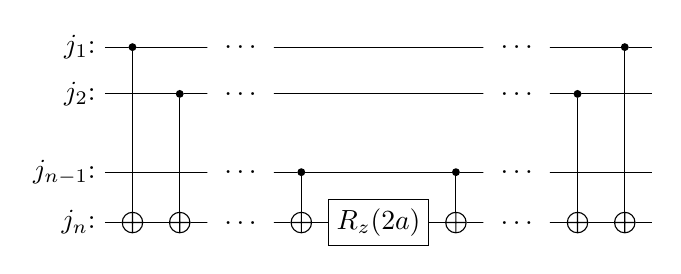
\begin{tikzpicture}
    \begin{yquant}
      qubit {$j_1\colon$} q[1];
      qubit {$j_2\colon$} q[+1];
      qubit {} q[+1]; discard q[2];
      qubit {$j_{n-1}\colon$} q[+1];
      qubit {$j_n\colon$} q[+1];
      cnot q[4] | q[0];
      cnot q[4] | q[1];
      text {$\ \ldots\ $} q[0,1,3,4];
      cnot q[4] | q[3];
      box {$R_z(2a)$} q[4];
      cnot q[4] | q[3];
      text {$\ \ldots\ $} q[0,1,3,4];
      cnot q[4] | q[1];
      cnot q[4] | q[0];
    \end{yquant}
  \end{tikzpicture}
  \fi
  \caption{Operaatori \(e^{-iZ_{j_1}Z_{j_2}\cdots Z_{j_n}a}\) realiseerimine kvantahelana~\cite{mansky+etal, nielsen+chuang}. Bitte, mis \(j_1\), \(j_2\), \(\cdots\), \(j_n\) hulgas ei esine, pole näidatud}
  \label{f:expz}
\end{figure}
Teisisõnu, bitile \(j_n\) tuleb järjest rakenda bittide \(j_1\), \(j_2\), \(\cdots\), \(j_{n-1}\) juhitud eitust.
Siis tuleb bitti \(j_n\) pöörata \(z\)-telje sihis nurga \(2a\) võrra.
Viimaks tuleb bitile \(j_n\) järjest rakendada bittide \(j_{n-1}\), \(j_{n-2}\), \(\cdots\), \(j_1\) juhitud eitusi.
Bitte, mis \(j_1\), \(j_2\), \(\cdots\), \(j_n\) hulgas ei esine, ei mõjutata.
Kesksele väravale \(R_z(2a)\) eelnev juhitud eituste osa arvutab bittide \(j_1\), \(j_2\), \(\cdots\), \(j_n\) paarsuse.
Keskne värav \(R_z(2a)\) teeb sobiva pöörde.
Järgnev juhitud eituste osa kustutab ära nüüdseks ebavajaliku informatsiooni paarsuse kohta~\cite{nielsen+chuang}.

Üldjuhul koosneb \(h_i\) nii Pauli \(I\) ja \(Z\) kui ka \(X\) ja \(Y\) operaatoritest, kuid \(h_i\) saab alati viia kujule~\eqref{eq:onlyz} rakendades sobivaid baasiteisendusi.
Vajalikud baasiteisendused on järgmised:
\begin{align}
    Z = HXH \rlap{,}\qquad Z = S^\dagger HYHS \rlap{.}
\end{align}

Näiteks juhul, kui
\begin{equation}
  h_i = Z_1X_2Y_3 \rlap{,}
\end{equation}
realiseerib operaatori \(e^{-i h_i t}\) ahel joonisel.

\begin{figure}[h]
  \centering
  \ifdefined\yquanton
  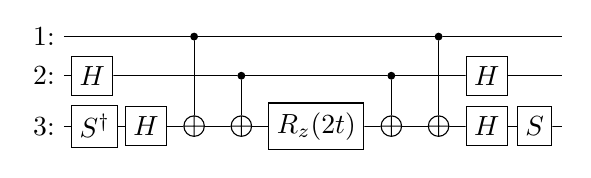
\begin{tikzpicture}
    \begin{yquant}
      qubit {$1\colon$} q[1];
      qubit {$2\colon$} q[+1];
      qubit {$3\colon$} q[+1];
      box {$H$} q[1];
      box {$S^{\dagger}$} q[2];
      box {$H$} q[2];
      cnot q[2] | q[0];
      cnot q[2] | q[1];
      box {$R_z(2t)$} q[2];
      cnot q[2] | q[1];
      cnot q[2] | q[0];
      box {$H$} q[1];
      box {$H$} q[2];
      box {$S$} q[2];
    \end{yquant}
  \end{tikzpicture}
  \fi
  \caption{Operaatori \(e^{-iZ_1X_2Y_3}\) realiseerimine kvantahelana.}
  \label{f:zxyex}
\end{figure}

Kokkuvõttes tuleb operaatori \(e^{-i t \sum_i h_i}\) realiseerimiseks kvantahelana gruppide kaupa järjestikku rakendada operaatoreid \(e^{-i h_i t/n}\) realiseerivaid kvantahelaid, kus \(n\) on piisavalt suur.
Näiteks, kui
\begin{align}\label{eq:hex}
    H=\frac{1}{3}X_1Y_1+\frac{2}{3}Z_1X_2 \rlap{,}
\end{align}
ja võtta trotterisammude arvuks \(n = 2\), siis realiseerib operaatori \(e^{-i Ht}\) ahel~\ref{fig:trot}.
Lõpliku trotterisammude arvu puhul on tegemist ligikaudse hinnanguga.

\begin{figure}
    \centering
    \ifdefined\yquanton
    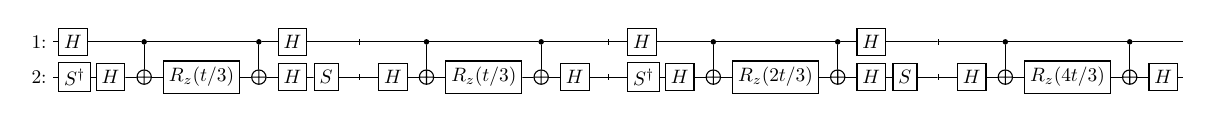
\begin{tikzpicture}[scale=0.7]
        \begin{yquant}
            qubit {$1\colon$} q[1];
            qubit {$2\colon$} q[+1];
            box {$H$} q[0];
            box {$S^\dagger$} q[1];
            box {$H$} q[1];
            cnot q[1] | q[0];
            box {$R_z(t/3)$} q[1];
            cnot q[1] | q[0];
            box {$H$} q[0];
            box {$H$} q[1];
            box {$S$} q[1];
            barrier q;
            box {$H$} q[1];
            cnot q[1] | q[0];
            box {$R_z(t/3)$} q[1];
            cnot q[1] | q[0];
            box {$H$} q[1];
            barrier q;
            box {$H$} q[0];
            box {$S^\dagger$} q[1];
            box {$H$} q[1];
            cnot q[1] | q[0];
            box {$R_z(2t/3)$} q[1];
            cnot q[1] | q[0];
            box {$H$} q[0];
            box {$H$} q[1];
            box {$S$} q[1];
            barrier q;
            box {$H$} q[1];
            cnot q[1] | q[0];
            box {$R_z(4t/3)$} q[1];
            cnot q[1] | q[0];
            box {$H$} q[1];
        \end{yquant}
    \end{tikzpicture}
    \fi
    \caption{Operaatori \(e^{-i\paren{\frac{1}{3}X_1Y_1+\frac{2}{3}Z_1X_2} t}\) realiseerimine kvantahelana.
    Joonisel on kaks operaatorite gruppi, mis vastab kahele trotterisammule.
    Igas grupis on omakorda kaks operaatorit}
    \label{fig:trot}
\end{figure}

\subsection{Juhitud ajalise arengu operaator}\label{sec:cu}

Faasihindamise jaoks on oluline, et unitaarne operaator oleks juhitud.
Juhitud ajalise arengu operaatori saab, kui seda realiseerivas kvantahelas asendada kõik pöörded juhitud pööretega.
Nõnda toiminud, sõltub iga Pauli sõne rakendamine sellest, mis on juhtkvantbiti olek.
Kui juhtkvantbitt on olekus \(\ket{0}\), pööre ei rakendu.
Et paarsuse arvutamine ja selle tagasi panemine on pöördoperatsioonid, siis kokkuvõttes antud Pauli sõne eksponent justkui ei rakendu.
Kui juhtkvantvitt on olekus \(\ket{1}\) pööre rakendub ja rakendub ka Pauli sõne eksponent tervikuna.
Joonisel~\ref{fig:trotexctrl} on näide juhitud ajalise arengu operaatorist, kui hamiltoniaan on antud valemiga~\eqref{eq:hex}.

\begin{figure}
    \centering
    \ifdefined\yquanton
    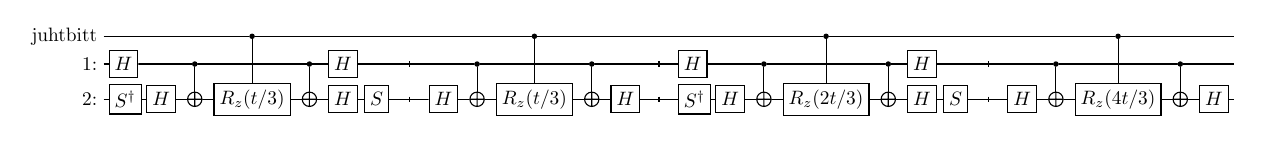
\begin{tikzpicture}[scale=0.7]
        \begin{yquant}
            qubit {juhtbitt} ctrl;
            qubit {$1\colon$} q[1];
            qubit {$2\colon$} q[+1];
            box {$H$} q[0];
            box {$S^\dagger$} q[1];
            box {$H$} q[1];
            cnot q[1] | q[0];
            box {$R_z(t/3)$} q[1] | ctrl[0];
            cnot q[1] | q[0];
            box {$H$} q[0];
            box {$H$} q[1];
            box {$S$} q[1];
            barrier q;
            box {$H$} q[1];
            cnot q[1] | q[0];
            box {$R_z(t/3)$} q[1] | ctrl[0];
            cnot q[1] | q[0];
            box {$H$} q[1];
            barrier q;
            box {$H$} q[0];
            box {$S^\dagger$} q[1] ;
            box {$H$} q[1];
            cnot q[1] | q[0];
            box {$R_z(2t/3)$} q[1] | ctrl[0];
            cnot q[1] | q[0];
            box {$H$} q[0];
            box {$H$} q[1];
            box {$S$} q[1];
            barrier q;
            box {$H$} q[1];
            cnot q[1] | q[0];
            box {$R_z(4t/3)$} q[1] | ctrl[0];
            cnot q[1] | q[0];
            box {$H$} q[1];
        \end{yquant}
    \end{tikzpicture}
    \fi
    \caption{Operaaatori \(e^{-i\paren{\frac{1}{3}X_1Y_1+\frac{2}{3}Z_1X_2} t}\) realiseerimine kvantahelana.}
    \label{fig:trotexctrl}
\end{figure}

Kui hamiltoniaanis esineb liige, mis on vaid ühikmaatriksite tensorkorrutis, tuleb seda eraldi arvestada.
Sellise liikme eksponent on globaalse faasi operaator, mille võib ajalise arengu operaatori, mis pole juhitud, juhul arvestamata jätta.
Samas juhitud globaalse faasi operaator rakendamine muudab suhtelist faasi ja seda peab arvestama.
Juhitud globaalse faasi operaatori võib asendanda juhtkvantbitil rakendatud suhtelise faasi operaatoriga, nagu näha joonisel~\ref{fig:globphase}, kus võrduse vasak ja parem pool on samaväärsed globaalse faasi täpsusega.

\begin{figure}[h]
    \centering
    \ifdefined\yquanton
    \begin{tikzpicture}
        \begin{yquantgroup}
            \registers{
                qubit {} q[2];
            }
            \circuit{
                box {\(GP(t)\)} q[1] | q[0];
            }
            \equals
            \circuit{
                box {\(P(-t)\)} q[0];
                barrier q[1];
            }
        \end{yquantgroup}
    \end{tikzpicture}
    \fi
    \caption{Juhitud globaalse faasi operaatori saab asendada juhtkvantbitile rakendatud faasi operaatoriga, mille argument peab olema vastupidine.}
    \label{fig:globphase}
\end{figure}

\chapter{Metoodika, tulemused ja arutelu}\label{chap:results}

Töö raames loodi programm, mille sisendiks on Jordan-Wigneri teisendustest saadud hamiltoniaan ja väljundiks kvantahel selle hamiltoniaani simuleerimiseks ja faasi hindamiseks.
See põhiprogramm liideti suuremasse programmi, mille sisendiks on molekulaarse süsteemi geomeetria ja väljunduks põhienergia hinnang.
Valmislahendusi kasutati vaid eelarvutusteks ning Jordan-Wigneri teisenduseks.
Loodud programmi kasutati vesiniku molekuli põhienergia leidmiseks.
Et siin töös ei võetud arvesse müra, siis viidi arvutused läbi kasutades kvantarvuti klassikalist simulaatorit.
Leiti sobivad parameetrid keemilise täpsuse saavutamiseks.
% ??? \(1{,}6\cdot10^{-3}\,{\rm Ha}\).

\section{Kasutatud vahendid}

Töös kasutati läbivalt programmeerimisekeelt Python (versioon 3.10.12).
Kvantahela koostamiseks ja selle klassikaliseks simuleerimiseks kasutati teeki Qiskit (versioon 1.0.0)~\cite{qiskit}.
Eelarvutusteks (molekulaarsete integraalide arvutamiseks) ja Jordan-Wigneri teisenduseks kasutati teeki OpenFermion (versioon 1.6.1)~\cite{openfermion}, mis omakorda kasutas kvantkeemiaprogrammi Psi4 (versioon 1.6.1)~\cite{psi4}.
Kasutatud arvuti protsessor oli 32 tuumaga AMD Ryzen Threadripper 3970X ja arvutil oli \(256\,{\rm GB}\) mälu.
Koostatud programm on kättesaadav veebis aadressil \url{https://github.com/mattiasmarka/peahamsim}.

\section{Keemiline baas}

Töös kasutati minimaalset keemilist baasi STO-3G, mis põhineb kolmel reaalsel Gaussi funktsioonil.
Baasis STO-3G on vesiniku molekuli jaoks neli spinnorbitaali, seega on faasi hindamise algoritmis seisundiregister nelja kvantbiti suurune.
Hartree-Focki seisund on kvantbittide ruumis
\begin{align}
  \ket{\text{HF}} = \ket{1100} \rlap{.}
\end{align}

\section{Parameetrite valik}

Töös taodeldi seda, et faasi hindamise algoritmi tulemus langeks keemilise täpsusega kokku täieliku koniguratsiooni vastasmõju (ingl FCI) meetodil arvutatud energiaga.
Tingimus selleks on
\begin{align}
  \abs{E_\text{PEA} - E_\text{FCI}} \le 0{,}0016\,{\rm Ha} \rlap{,}
\end{align}
kus \(E_\text{PEA}\) on faasi hindamise algoritmi tulemusel saadud energia, \(E_\text{FCI}\) on täieliku konfiguratsiooni vastasmõju meetodil arvutatud energia.

Keemilise täpsuse saavutamiseks vajalik trotterisammude arv ja faasi hindamise algoritmi tööregistri suurus määrati eksperimentaalselt.
Joonisel~\ref{fig:bitstrots} on näha energia vea sõltuvus tööregistri suurusest erinevate trotterisammude arvude jaoks.
Sidemepikkusel \(0{,}75\,{\rm Å}\), mis vastab tasakaalugeomeetriale (vt järgmine jaotis), on keemilise täpsuse saavutamiseks vajalik minimaalselt kolm trotterisammu ja kümme tööbitti.
Energia tõkkena kasutati väärtust \(2\,{\rm Ha}\).
Edaspidi on kõik arvutused läbi viidud just nende parameetritega.

\begin{figure}[h]
  \centering
  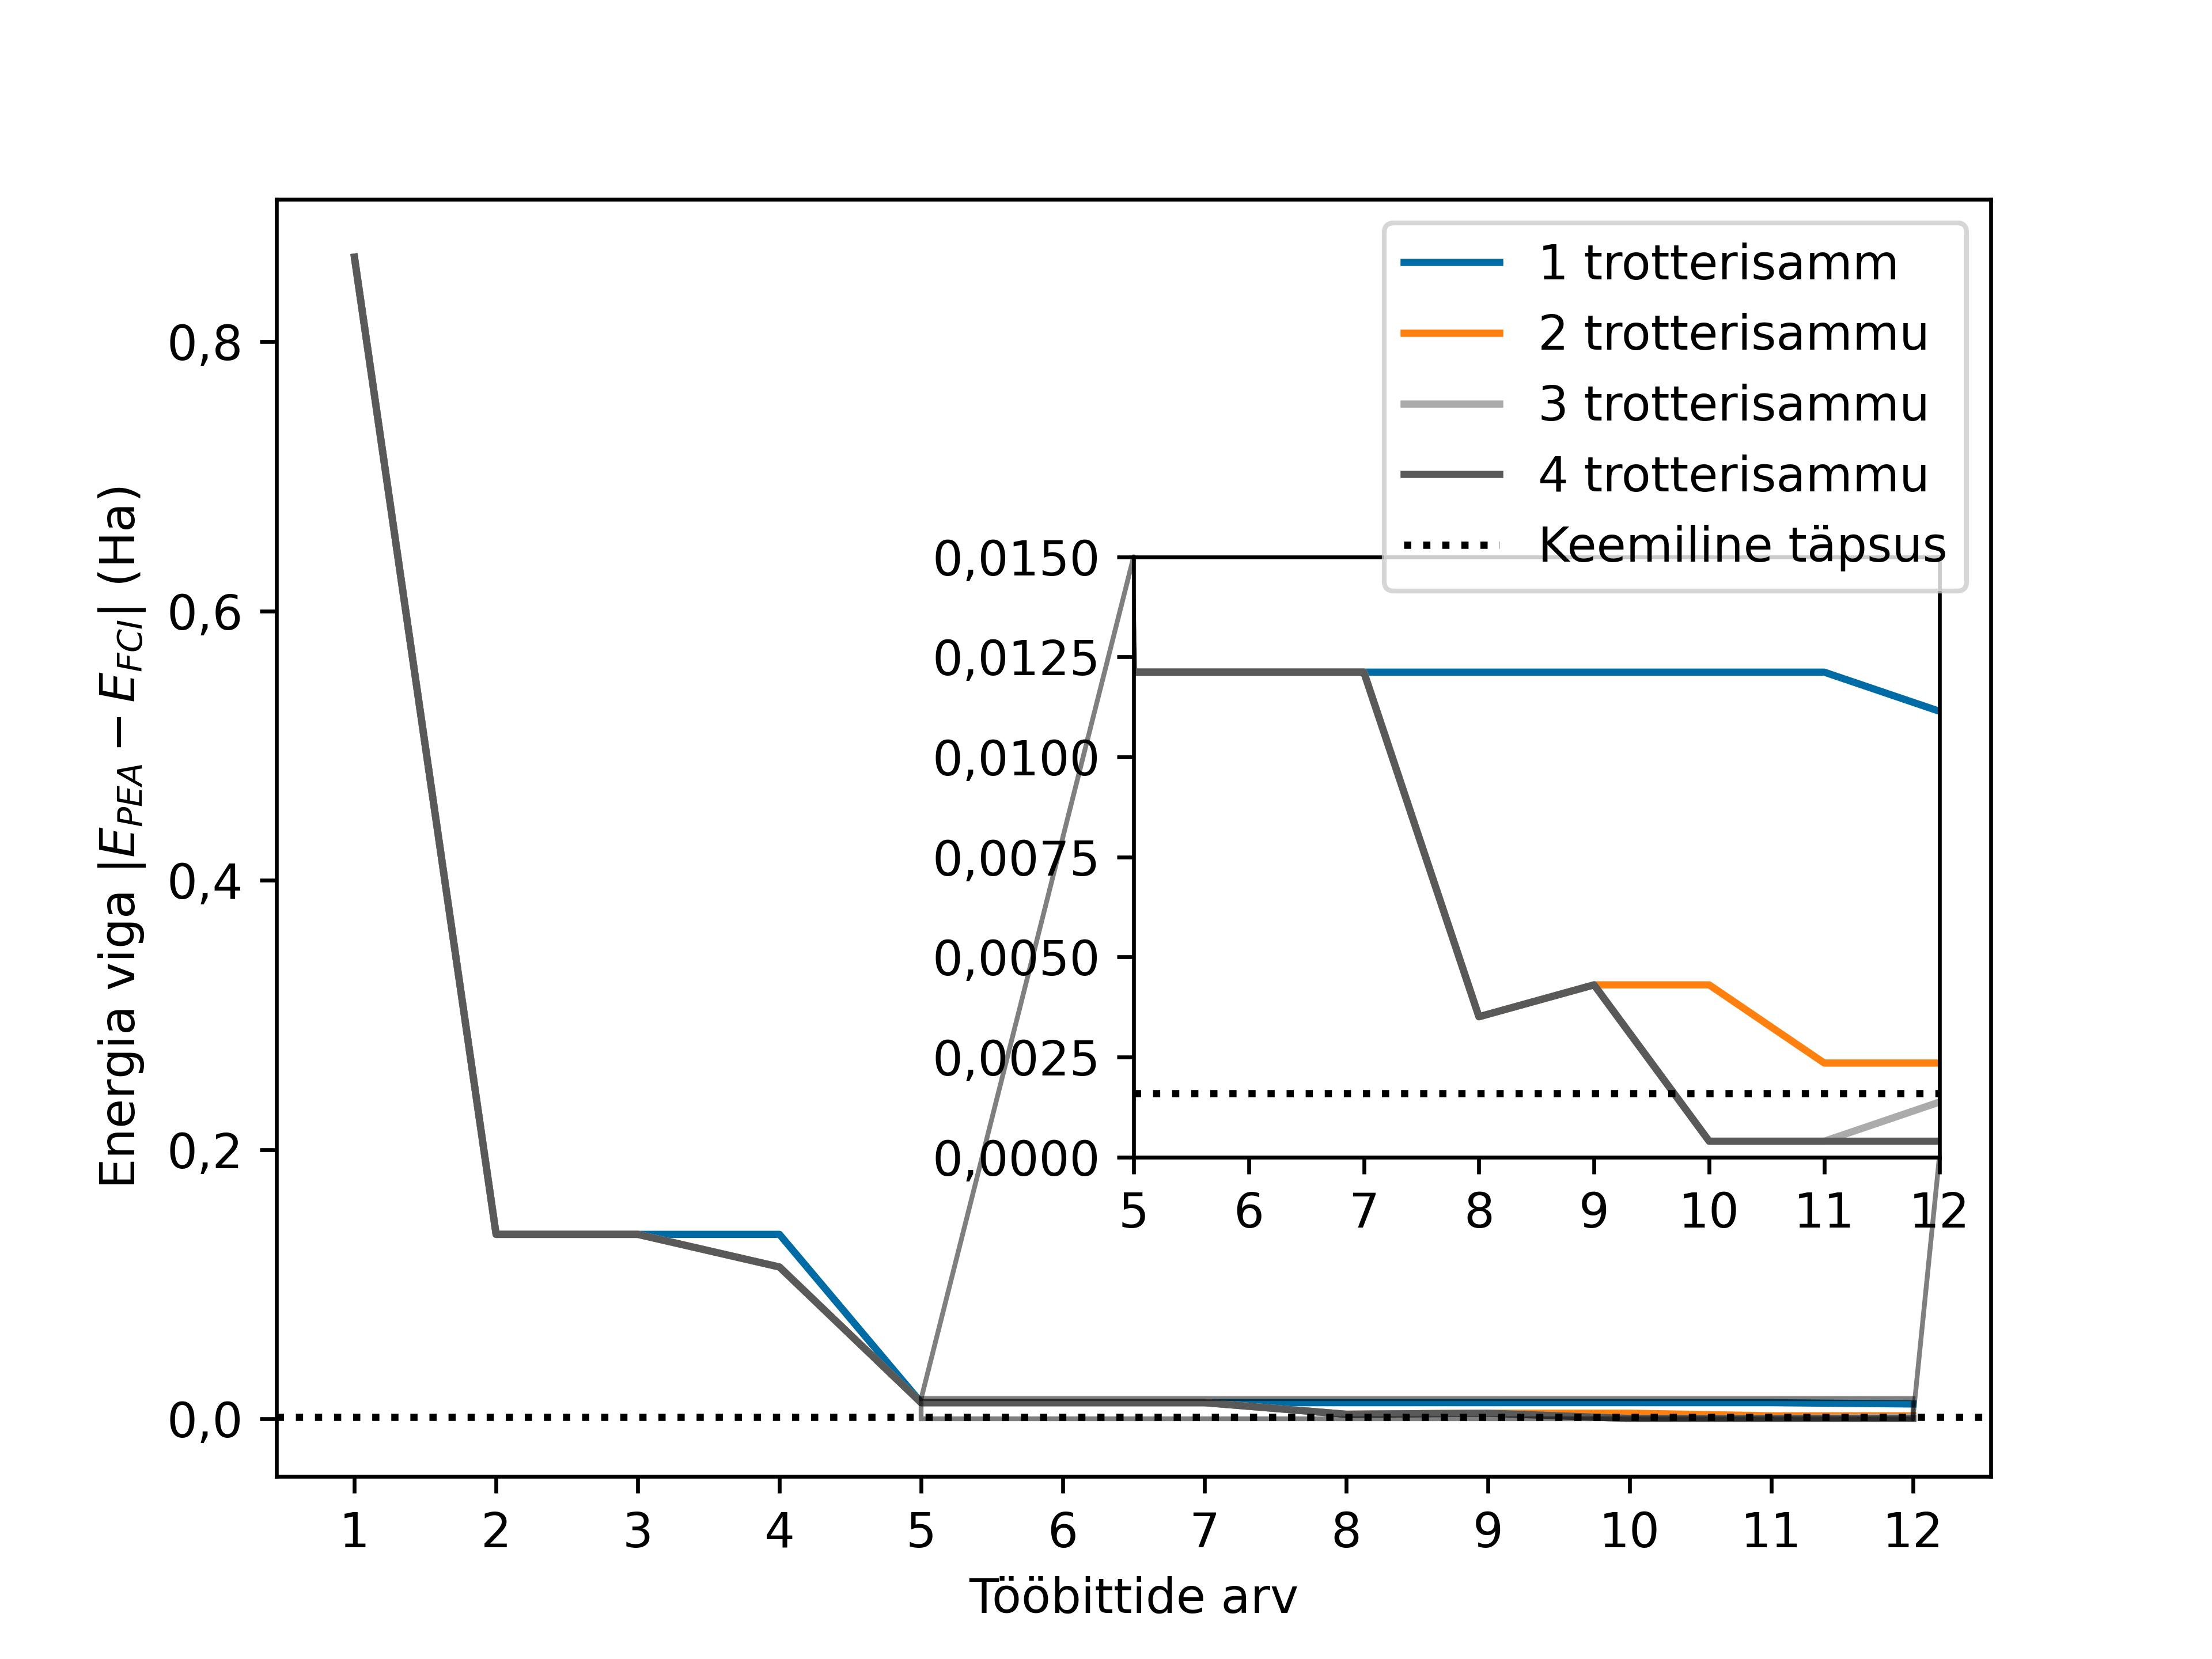
\includegraphics[width=.65\hsize]{bitstrots.jpg}
  \caption{Energia vea sõltuvus faasi hindamise tööbittide arvust erinevate trotterisammude arvude jaoks}
  \label{fig:bitstrots}
\end{figure}

\begin{figure}[h]
  \centering
  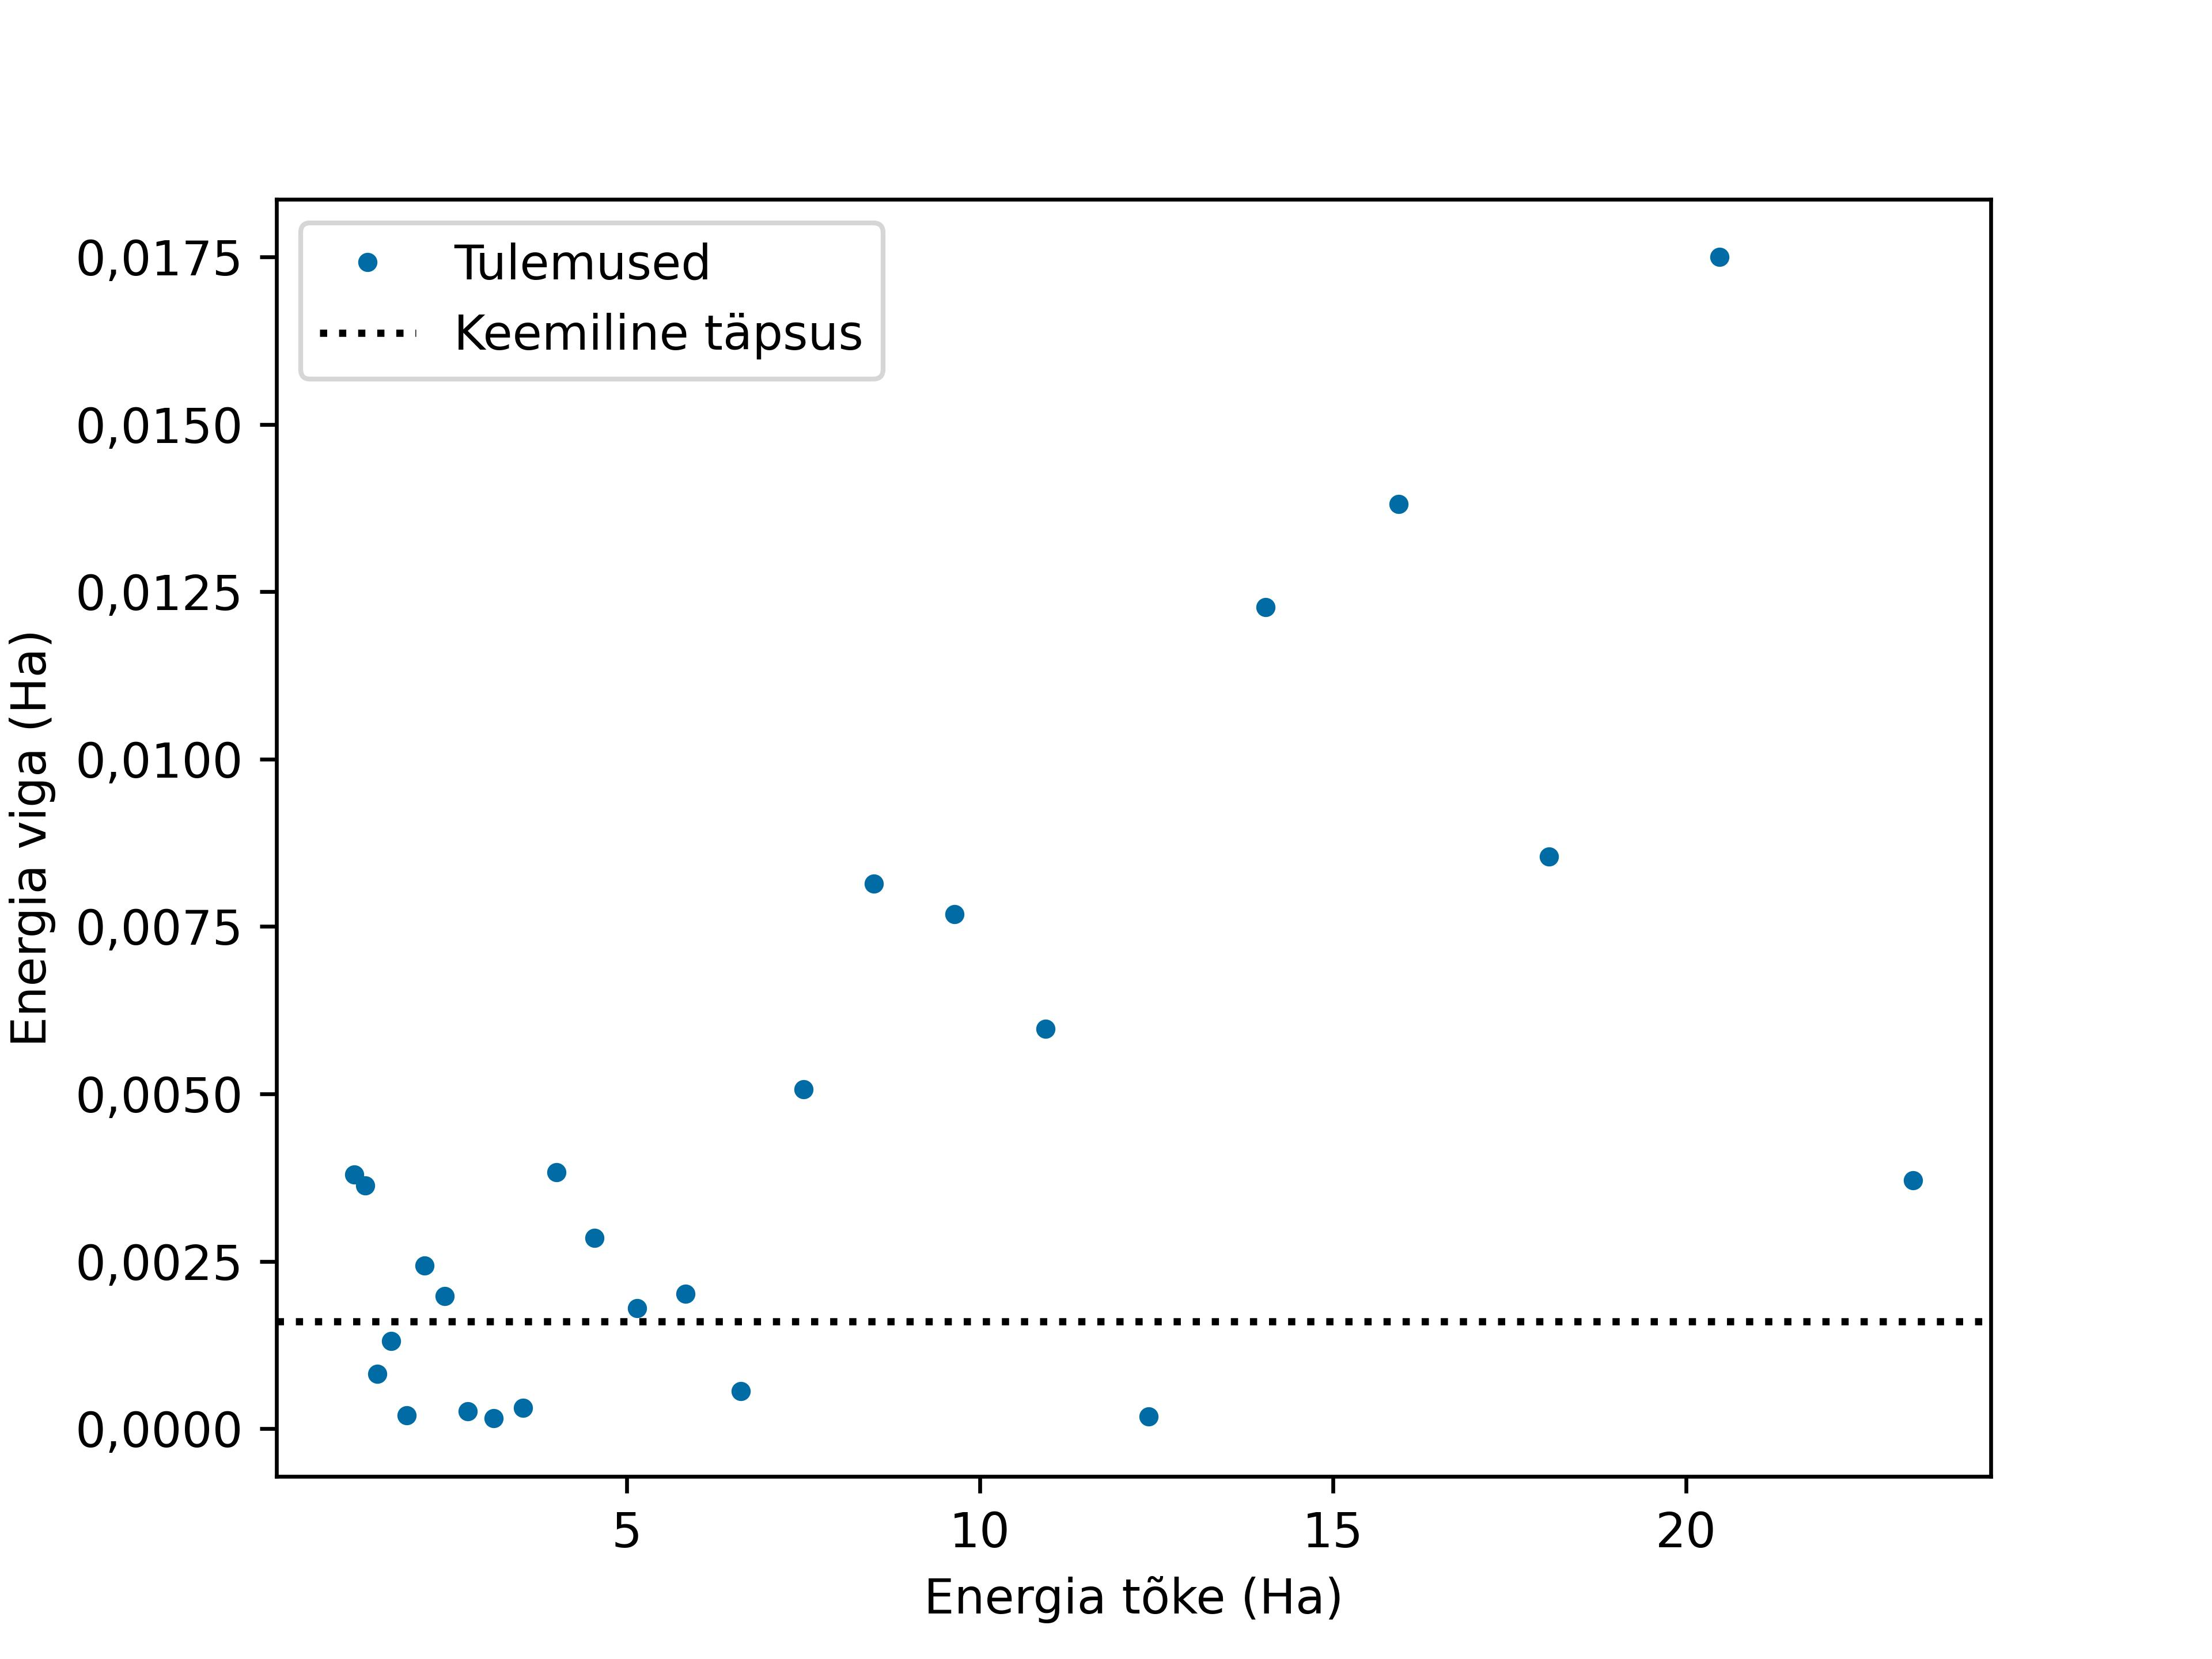
\includegraphics[width=.65\hsize]{bounds.jpg}
  \caption{Energia vea sõltuvus energia tõkke valikust.}
  \label{fig:bounds}
\end{figure}

Energia hinnangu täpsust mõjutab ka energia tõkke valik, mida kujutab joonis~\ref{fig:bounds}.
Üldine seaduspära on, et mida suurem on tõke võrreldes energiaga, mida hinnatakse, seda ebatäpsem on hinnang.
Seega tuleks energia tõke valida võimalikult väike.

\section{Tulemused}

Töö põhitulemuseks on vesiniku molekuli põhienergia sõltuvus sidemepikkusest, mis on kujutatud joonisel~\ref{fig:scan}.
Võrdluseks on toodud täieliku konfiguratsiooni vastasmõju  meetodil arvutatud energiad.
Energiad on arvutatud sidemepikkustel \(0{,}25 \ldots 2{,}85\,{\rm Å}\).
Hamiltoniaani simuleermiseks on kasutatud kolme trotterisammu ja faasi hindamiseks kümmet tööbitti.

Jooniselt~\ref{fig:scan} on näha, et minimaalne energia on põhiolekul siis, kui sidemepikkus on \(0{,}75\,{\rm Å}\).
Sellel pikkusel on faasi hindamise algoritmi põhjal energia \(-0{,}1367\,{\rm Ha}\), täieliku konfiguratsiooni vastasmõju meetodil \(-0{,}1371\,{\rm Ha}\),
seega kahel meetodil arvutatud energiate erinevus on väiksem kui keemiline täpsus.

Samas on joonisel~\ref{fig:scan} veel näha, et sidemepikkustel \(2{,}55\,{\rm Å}\) ja \(2{,}60\,{\rm Å}\) ei langes faasi hindamise algoritmi tulemused kokku täieliku konfiguratsiooni vastasmõju meetodil arvutatud energiatega.
Tegemist on olukordadega, kus kolm trotterisammu on hamiltoniaani simuleerimiseks liiga vähe.

\begin{figure}[h]
  \centering
  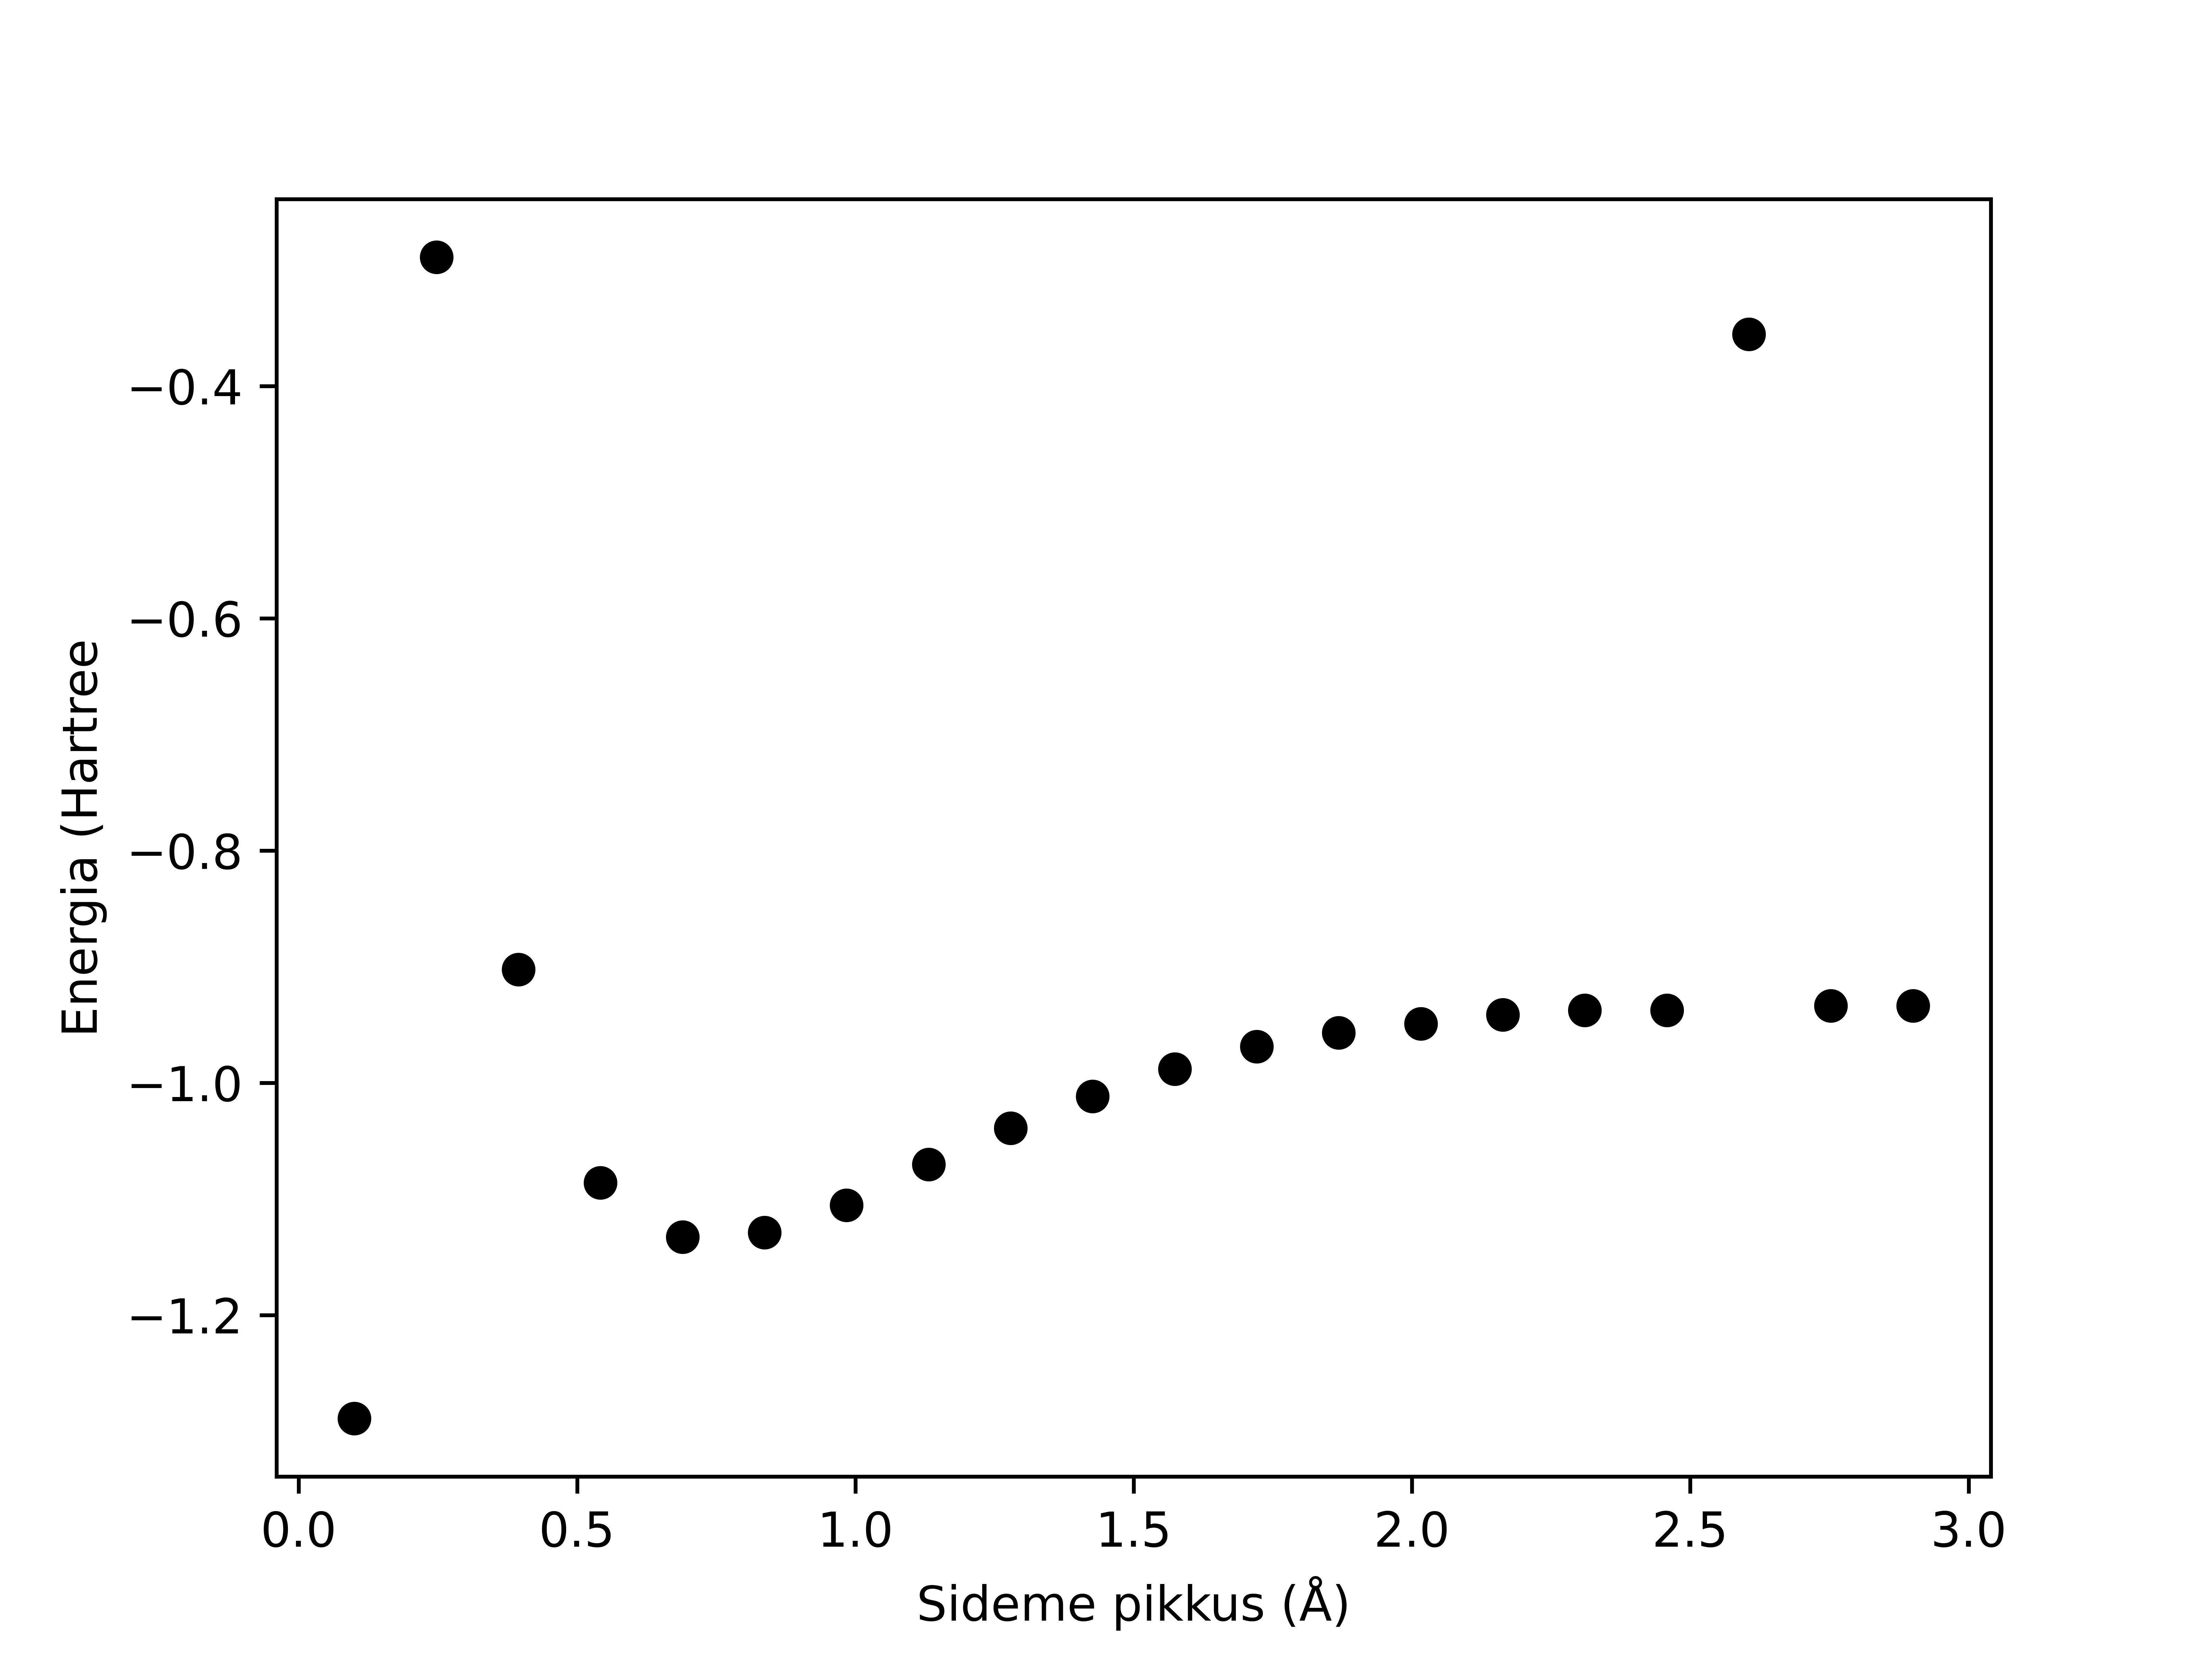
\includegraphics[width=.65\hsize]{scan.jpg}
  \caption{Põhienergia sõltuvus sidemepikkusest. Pidev joon on täieliku konfiguratsiooni vastasmõju meetodil arvutatud energia. Punktid on faasi hindamise meetodil arvutatud energiad.}
  \label{fig:scan}
\end{figure}

\section{Arutelu}\label{chap:discussion}

Selle töö kirjutamise ajal ei olnud võimalik arvutusi, mis on vajalikud vesiniku molekuli keemiliselt täpse põhienergia leidmiseks, läbi viia kvantarvutil.
Seda piiras kvantarvutite ebatäiuslik riistvara.

Kvantarvutite rääkides tehakse vahet füüsilistel ja loogilistel kvantbittidel.
Füüsiline kvantbitt on füüsikaline süsteem, mille mudeliks on loogiline kvantbitt.
Kõrvalistest mõjudest häirituna ei käitu füüsiline kvantbitt kunagi nagu loogiline kvantbitt.
Samas arvestatakse kvantalgoritme luues just loogiliste kvantbittidega.
Seega on oluline, et füüsilised kvantbitid oleksid piisavalt täiuslikud, et neid võiks vaadata loogiliste kvantbittidena.

Praeguse perioodi kohta kvantarvutite arengus kasutatakse lühendit NISQ (noisy inter\-me\-diate-scale quantum)~\cite{preskill}.
Olemas on küll juba mõnesaja füüsilise kvantbitiga kvantarvutid, kuid need on mürarikkad.
See asjaolu piirab kvantarvutite kasutamise paljude ülesannete lahendamiseks.

Kvantarvutite arengu järgmise perioodi kohta, millal neid saaks kasutada ka suurt hulka loogilisi kvantbitte nõudvate ülesannete lahendamiseks, kasutatakse lühendit FTQC (fault-tolerant quantum computing).
Kvantarvutite riistvara arendamisega tegelevad organisatsioonid on võtnud eesmärgiks 2020ndate aastate lõpuks jõuda selle perioodi lävele~\cite{ibmq+roadmap, quera+roadmap}.
Esimesed sammud selle eesmärgi suunas on juba tehtud: Quera töörühmal õnnestus realiseerida 48 loogilist kvantbitti~\cite{quera}.

Siin töös esitatud viisil vesiniku molekuli põhienergia arvutamiseks keemilise täpsusega oleks vaja kvantarvutit, millel on \(10 + 4\) loogilist kvantbitti.
Töö tegijatele selliste kvantarvutit kasutada polnud.

Kummatigi ei saa öelda, et kvantarvuti kasutamine vesiniku põhienergia arvutamise keemilise täpsusega oleks töö kirjutamise hetkel olnud võimatu.
Nimelt on teada mitu lahendamis\-algoritmi, mis sobivad ka NISQ-perioodil kasutamiseks.
Üks näide on variatsioonilise lahendamise algoritm~\cite{omalley+etal, raidlo}.
Teine on  iteratiivne faasi hindamise algoritm, mis põhineb klassikalise ja kvantarvuti koostööl~\cite{omalley+etal}.
Et iteratiivne faasi hindamise algoritm on saadud siin töös esitatud tavalise faasi hindamise algoritmi kohandamisel, siis on faasi hindamise algoritm relevantne ka praegusel NISQ-perioodil.
Kvantarvutusressursside säästmiseks tasub ka uurida, kas hamiltoniaani on enne simuleerimist võimalik lihtsustada, nagu on näiteks teinud O'Malley jt~\cite{omalley+etal}.
Kokkuvõttes on vähemalt kaks suunda antud töö edasi arendamiseks: üks on kasutada iteratiivset faasi hindamise algoritmi, teine on lihtsustada hamiltoninaani kvantarvutusressurside säästmiseks.

\chapter{Kokkuvõte}

Töös tutvustati faasi hindamise algoritmil põhinevat kvantarvutusliku meetodit molekulaarse hamiltoniaani põhienergia leidmiseks, mille kasutamist motiveerib selle klassikalisest parem efektiisus.
Käsitleti ülesande kõiki lahendamisetappe pöörates erilist tähelepanu hamiltoniaani simuleerimisele ja faasi hindamisele.
Koostati programm põhienergia leidmiseks ja rakendati seda vesiniku molekuli jaoks.

Esimeses peatükis käsitleti lahendamise eelarvutusi.
Alustuseks pandi kirja molekulaarse süsteemi üldine hamiltoniaan~--- molekulaarne hamiltoniaan.
Siis kasutati Born-Oppeheimeri lähendust, et molekulaarset hamiltoniaani lihtustada, jõudes nii vaid elektornkatet kirjeldava hamiltoniaanini~--- elektroonilise hamiltoniaanini.
Järgmisena käsitleti Slateri determinantide kasutamist lainefunktsiooni esitamiseks.
Anti ülevaade, kuidas Hartree-Focki lähendus lubab leida Slateri determinantides esinevad spinnorbitaalid.
Kõige viimaks näidati, et eelarvutuste käigus tuleb leida molekulaarsed integraalid, mis on vajalikud ülesande esitamiseks edasiseks lahendamiseks sobivamal teise kvantiseerimise kujul.

Teise peatüki teemaks olid lahendamise põhiarvutused.
Esmalt tutvustati faasi hindamise algoritmi.
Eraldi pöörati tähelepanu faasi hindamise algoritmi kasutamisele hamiltoniaani omaväärtuste leidmiseks.
Teiseks käsitleti hamiltoniaani simuleerimist.
Hamiltoniaani kujutamiseks kvantbittide ruumi kasutati Jordan-Wigneri teisendust.
Kvantbittide ruumi hamiltoniaani põhjal koostati ajalise arengu operaator, mille realiseerimiseks kvantahealana kasutati trotteriseerimist ja treppalgoritmi.

Kolmandas peatükis käsitleti vesiniku molekuli põhienergia leidmiseks kasutatud tehnilisi vahendeid ja parameetrite valikut.
Tehti kindlaks, et keemilise täpsuse saavutamiseks on tarvis minimaalselt kolm trotterisammu ja kümme faasi hindamise tööregistri kvantbitti.
Arvutused viidi läbi kasutades kvantarvuti simulaatorit, kuid käsitleti ka arvutuste läbiviimise võimalikkust kvantarvutil.
Jõuti järelduseni, et hetkel ei saa veel töös esitatud meetodil arvutuste läbiviimiseks kasutada kvantarvutid piisava arvu loogiliste kvantbittide puudumise tõttu.
Viimaks juhiti tähelepanu kahele alternatiivsele meetodile (variatsioonilisele kvantlahendamisele ja iteartiivsele faasi hindamisele), mida saab juba praegu kasutada vesiniku molekuli põhienergia leidmiseks kvantarvutil.

\printbibliography[heading=bibintoc, title=Kirjandus]

\end{document}
